%%%%%%%%%%%%%%%%%%%%%%%%%%%%%%%%%%%%%%%%%%%%%%%
%
% Template per Elaborato di Laurea
% DISI - Dipartimento di Ingegneria e Scienza dell’Informazione
%
% update 2015-09-10
%
% Per la generazione corretta del 
% pdflatex nome_file.tex
% bibtex nome_file.aux
% pdflatex nome_file.tex
% pdflatex nome_file.tex
%
%%%%%%%%%%%%%%%%%%%%%%%%%%%%%%%%%%%%%%%%%%%%%%%

% formato FRONTE RETRO
\documentclass[epsfig,a4paper,11pt,titlepage,twoside,openany]{book}
\usepackage{verbatim}
\usepackage{epsfig}
\usepackage{plain}
\usepackage{setspace}
%\usepackage[paperheight=29.7cm,paperwidth=21cm,outer=1.5cm,inner=2.5cm,top=2cm,bottom=2cm]{geometry} % per definizione layout
\usepackage{hyperref}
\usepackage[paperheight=29.7cm,paperwidth=21cm,left=3cm,right=3cm,top=2cm,bottom=2cm]{geometry} % per definizione layout

\usepackage{titlesec} % per formato custom dei titoli dei capitoli

%%%%%%%%%%%%%%
% supporto lettere accentate
%
%\usepackage[latin1]{inputenc} % per Windows;
\usepackage[utf8x]{inputenc} % per Linux (richiede il pacchetto unicode);
%\usepackage[applemac]{inputenc} % per Mac.

\singlespacing

\usepackage[english]{babel}

%Color
\usepackage[dvipsnames]{xcolor}
%Code section
\usepackage{listings}
\usepackage{color}

\definecolor{dkgreen}{rgb}{0,0.6,0}
\definecolor{gray}{rgb}{0.5,0.5,0.5}
\definecolor{mauve}{rgb}{0.58,0,0.82}

\lstset{frame=tb,
  language=C,
  aboveskip=3mm,
  belowskip=3mm,
  showstringspaces=false,
  columns=flexible,
  basicstyle={\small\ttfamily},
  numbers=none,
  numberstyle=\tiny\color{gray},
  keywordstyle=\color{blue},
  commentstyle=\color{dkgreen},
  stringstyle=\color{mauve},
  breaklines=true,
  breakatwhitespace=true,
  tabsize=3
}

%image position
\usepackage{float}

%table
\usepackage{array}

\begin{document}

  % nessuna numerazione
  \pagenumbering{gobble} 
  \pagestyle{plain}

\thispagestyle{empty}

\begin{center}
  \begin{figure}[h!]
    \centerline{
\psfig{file=marchio_unitrento_colore_it_202002.eps,width=0.6\textwidth}}
  \end{figure}

  \vspace{2 cm} 

  \LARGE{Dipartimento di Ingegneria e Scienza dell’Informazione\\}

  \vspace{1 cm} 
  \Large{Corso di Laurea\\
    %Informatica
    %Ingegneria dell'Informazione e delle Comunicazioni
    %Ingegneria dell'Informazione e Organizzazione d'Impresa
    %Ingegneria Elettronica e delle Telecomunicazioni
    Ingegneria Informatica, delle Telecomunicazioni ed Elettronica
  }

  \vspace{2 cm} 
  \Large\textsc{Elaborato finale\\} 
  \vspace{1 cm} 
  \Huge\textsc{TITLE\\}
  \Large{\it{Sottotitolo}}


  \vspace{2 cm} 
  \begin{tabular*}{\textwidth}{ c @{\extracolsep{\fill}} c }
  \Large{Supervisore} & \Large{Laureando}\\
  \Large{......}& \Large{......}\\
  \end{tabular*}

  \vspace{2 cm} 

  \Large{Anno accademico .../...}
  
\end{center}



  \clearpage
 
%%%%%%%%%%%%%%%%%%%%%%%%%%%%%%%%%%%%%%%%%%%%%%%%%%%%%%%%%%%%%%%%%%%%%%%%%%
%%%%%%%%%%%%%%%%%%%%%%%%%%%%%%%%%%%%%%%%%%%%%%%%%%%%%%%%%%%%%%%%%%%%%%%%%%
%% Nota
%%%%%%%%%%%%%%%%%%%%%%%%%%%%%%%%%%%%%%%%%%%%%%%%%%%%%%%%%%%%%%%%%%%%%%%%%%
%% Sezione Ringraziamenti opzionale
%%%%%%%%%%%%%%%%%%%%%%%%%%%%%%%%%%%%%%%%%%%%%%%%%%%%%%%%%%%%%%%%%%%%%%%%%%
%%%%%%%%%%%%%%%%%%%%%%%%%%%%%%%%%%%%%%%%%%%%%%%%%%%%%%%%%%%%%%%%%%%%%%%%%%
  \thispagestyle{empty}

\begin{center}
  {\bf \Huge Acknowledgments}
\end{center}

\vspace{4cm}
\emph{I  would like to thank my supervisors Prof. Kasim Sinan Yildirim, Prof. Davide Brunelli and Alessandro Torrisi for their help and advice with this thesis.\\
I would also like to thank my family that always supported me.}


  
  


  \clearpage
  \pagestyle{plain} % nessuna intestazione e pie pagina con numero al centro

  
  % inizio numerazione pagine in numeri arabi
  \mainmatter

%%%%%%%%%%%%%%%%%%%%%%%%%%%%%%%%%%%%%%%%%%%%%%%%%%%%%%%%%%%%%%%%%%%%%%%%%%
%%%%%%%%%%%%%%%%%%%%%%%%%%%%%%%%%%%%%%%%%%%%%%%%%%%%%%%%%%%%%%%%%%%%%%%%%%
%% Nota
%%%%%%%%%%%%%%%%%%%%%%%%%%%%%%%%%%%%%%%%%%%%%%%%%%%%%%%%%%%%%%%%%%%%%%%%%%
%% Si ricorda che il numero massimo di facciate e' 30.
%% Nel conteggio delle facciate sono incluse 
%%   indice
%%   sommario
%%   capitoli
%% Dal conteggio delle facciate sono escluse
%%   frontespizio
%%   ringraziamenti
%%   allegati    
%%%%%%%%%%%%%%%%%%%%%%%%%%%%%%%%%%%%%%%%%%%%%%%%%%%%%%%%%%%%%%%%%%%%%%%%%%
%%%%%%%%%%%%%%%%%%%%%%%%%%%%%%%%%%%%%%%%%%%%%%%%%%%%%%%%%%%%%%%%%%%%%%%%%%

    % index
    \tableofcontents
    \clearpage
    
    
          
    % gruppo per definizone di successione capitoli senza interruzione di pagina
    \begingroup
      % nessuna interruzione di pagina tra capitoli
      % ridefinizione dei comandi di clear page
      \renewcommand{\cleardoublepage}{} 
      \renewcommand{\clearpage}{} 
      % redefinizione del formato del titolo del capitolo
      % da formato
      %   Capitolo X
      %   Titolo capitolo
      % a formato
      %   X   Titolo capitolo
      
      \titleformat{\chapter}
        {\normalfont\Huge\bfseries}{\thechapter}{1em}{}
        
      \titlespacing*{\chapter}{0pt}{0.59in}{0.02in}
      \titlespacing*{\section}{0pt}{0.20in}{0.02in}
      \titlespacing*{\subsection}{0pt}{0.10in}{0.02in}
      
      % sommario
      \chapter*{Abstract} % senza numerazione
\label{summary}

\addcontentsline{toc}{chapter}{Abstract} % da aggiungere comunque all'indice
The use of battery-free systems is a revolutionary frontier for the Internet of Things; in fact, it allows network nodes to be unconstrained by the use of batteries.\\
To achieve this, battery-free systems use ambient energy to charge a capacitor and use it as a power source. Because of the unpredictability of environmental energy sources, the node is often subject to power failure.
Communication then becomes intermittent and data loss particularly frequent.\\
To solve this problem, we implemented a tiny communication stack that implements non-volatile memory management for data storage and the TRAP protocol for energy awareness between nodes.
\newpage



%%%%%%%%%%%%%%%%%%%%%%%%%%%%%%%%%%%%%%%%%%%%%%%%%%%%%%%%%%%%%%%%%%%%%%%%%%
%%%%%%%%%%%%%%%%%%%%%%%%%%%%%%%%%%%%%%%%%%%%%%%%%%%%%%%%%%%%%%%%%%%%%%%%%%
%% Nota
%%%%%%%%%%%%%%%%%%%%%%%%%%%%%%%%%%%%%%%%%%%%%%%%%%%%%%%%%%%%%%%%%%%%%%%%%%
%% Sommario e' un breve riassunto del lavoro svolto dove si descrive 
%% l’obiettivo, l’oggetto della tesi, le metodologie e 
%% le tecniche usate, i dati elaborati e la spiegazione delle conclusioni 
%% alle quali siete arrivati.
%% Il sommario dell’elaborato consiste al massimo di 3 pagine e deve contenere le seguenti informazioni: 
%%   contesto e motivazioni
%%   breve riassunto del problema affrontato
%%   tecniche utilizzate e/o sviluppate
%%   risultati raggiunti, sottolineando il contributo personale del laureando/a
%%%%%%%%%%%%%%%%%%%%%%%%%%%%%%%%%%%%%%%%%%%%%%%%%%%%%%%%%%%%%%%%%%%%%%%%%%
%%%%%%%%%%%%%%%%%%%%%%%%%%%%%%%%%%%%%%%%%%%%%%%%%%%%%%%%%%%%%%%%%%%%%%%%%%      
      
      %%%%%%%%%%%%%%%%%%%%%%%%%%%%%%%%
      % lista dei capitoli
      %
      % \input oppure \include
      %
      \chapter{Introduction}
\label{cha:intro}
This thesis contains all the work done to implement a tiny network stack for battery-free communication.\\
The microcontroller family used in this project is MSP430. These microcontrollers are built on a 16-bit processor that provides low power consumption.\\
Before looking in detail at what has been implemented, it is worthwhile to provide some background information to introduce the current situation of battery-free communication.\\
\section{Battery-Free Devices}
\label{sec:batteryFreeDevices}
The use of distributed sensors in the environment is a very interesting frontier for IoT applications; however, it is impossible to think of being able to wire all connections.\\
For this reason Wireless Sensor Networks (WSNs), distributed networks of sensors that communicate wirelessly, are being introduced.\\
In recent years processors are becoming less energivorous and batteries more durable but thinking about a sensor network that relies on batteries does not seem the best solution.
Batteries need to be replaced periodically \cite{BatteryDegradation}, and this is complicated if the nodes are in environments that are difficult or unsafe to reach.\\
To make the nodes energy-autonomous, researchers are working on systems that harvest energy from the environment in a capacitor to use as a power source; some examples of energy are solar \cite{7479815}, RF \cite{article} , kinetic \cite{KineticEnergy}, thermal \cite{ThermalEnergy} and some  bacteria species \cite{10.1145/3362053.3363491}.\\
In this way, there is no need to rely on batteries, and the system can work for its entire lifetime without \cite{ManteinanceWSN} or with minimal maintenance.\\
The energy harvested by these devices is employed to produce and get data from external sources, process it, and send it to other nodes in the network.\\
The operation of these devices is closely related to environmental conditions, and it is not guaranteed to always have sufficient energy to perform all the intended tasks. \\
Because of this low reliability of the energy level for task completion, nodes are prone to power failures and consequently work intermittently.\\ 
The frequency of these outages depends on many factors, such as capacitor size, available energy in the environment, and node consumption.\\
\section{Problem Statement}
\label{sec:problemStatement}
Stored energy is precious and should not be wasted. If a node transmits a packet and the receiving side does not have enough energy to finish receiving, the packet is lost, and there is a power failure on the node (Figure \ref{fig:TransmissionProblem}).
Power failures can have many other causes such as producing a data item without first verifying the availability of energy for proper production or suddenly consuming more energy than expected.
\\Anyway, in the event of a power failure, the node loses all the data it had produced and must consume more energy to produce the data again. At the same time, data received from other nodes in the network are lost. The latter scenario presents a considerable waste of energy; in fact, the energy used to produce, send and receive the packet is wasted.\\
To avoid these problems we need to:
\begin{enumerate}
\item Save data in non-volatile memory so that nothing is lost in case of power failure
\item Resume data management to just before power failure
\item Recognize expired data and delete them
\end{enumerate}
These problems must be solved in a way that provides the application layer with the methods of producing/sending and receiving data while hiding their complexity from the end user.
\begin{figure}[ht]
\centerline{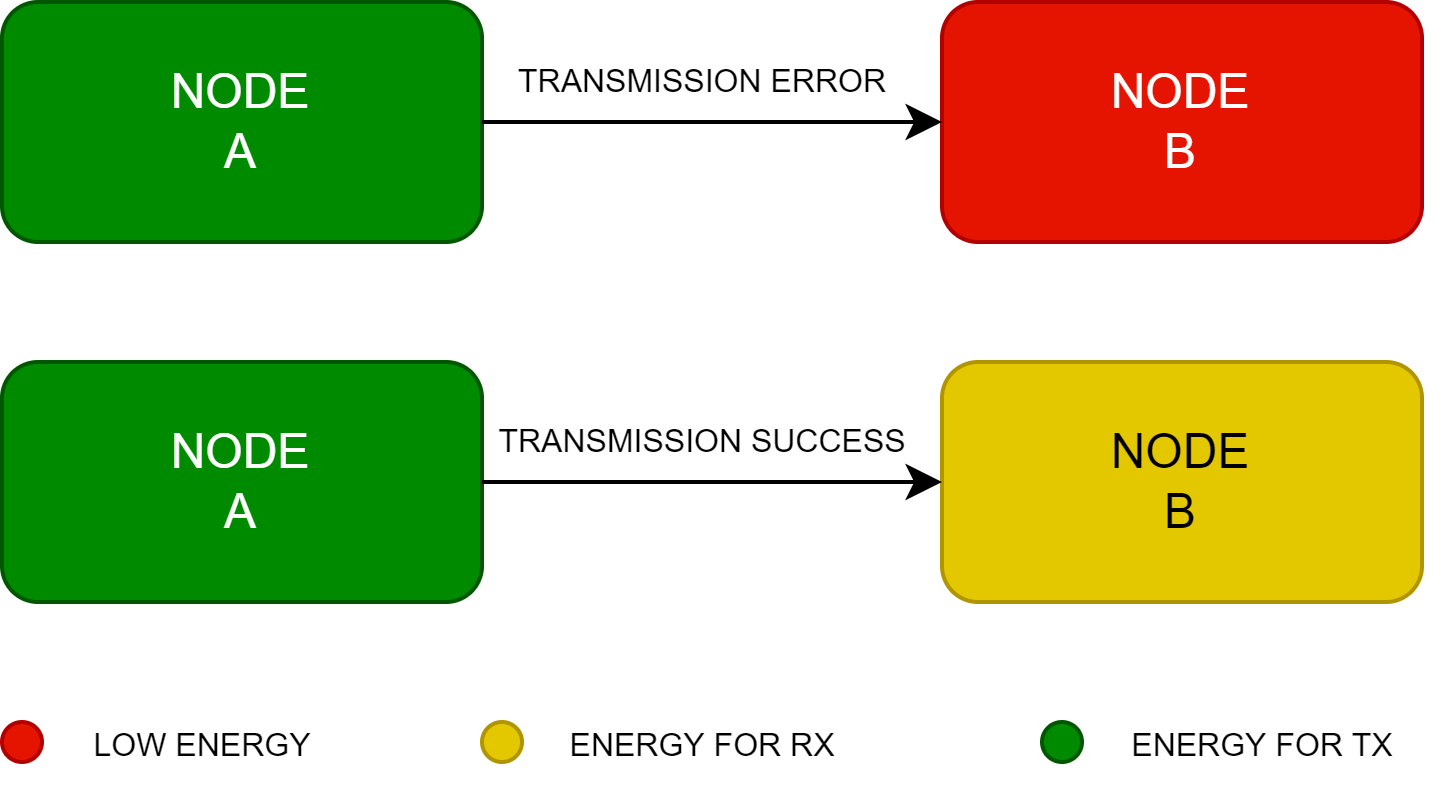
\psfig{file=Images/TransmissionProblem.png,width=0.6\textwidth}}
\caption{\footnotesize \centering Transmission examples}
\label{fig:TransmissionProblem}
\end{figure}
\section{Contributions}
\label{sec:contributions}
There are methodologies to limit power failures, such as the TRAP protocol \cite{9733918}, but it is impossible to be certain that they will not happen. Therefore, the contributions of this thesis are to present a Communication Stack for battery-free communication that:
\begin{enumerate}
\item Implements the TRAP protocol \cite{9733918} to be aware of the energy level of neighboring nodes
\item Saves data received from the Application Layer in non-volatile memory
\item Saves data received from the Physical Layer in non-volatile memory
\item Recovers data from memory in cases of power failure
\item Delete expired data to avoid unnecessary sending or processing
\item Send and receive data to and from Application Layer
\item Send and receive data to and from Physical Layer
\end{enumerate}
In addition to the problems that the stack aims to solve, we want a system that is modular and easily scalable.\\
In particular, the stack must be easily usable by the Application Layer and easily usable by the Physical Layer even when there are a large number of nodes in the network.\\
The Physical Layer must also not be binding on the stack, which must be able to work with different communication technologies, such as RF Backscatter communication \cite{transientComp} or VLC communication \cite{VLCCOmm}, by changing only the Physical Layer.\\
For these reasons, the nonfunctional requirements of the stack are:
\begin{itemize}
    \item Scalability
    \item Modularity
\end{itemize}
  

\newpage
      \chapter{System Design}
\label{cha:System Architecture}
This thesis work aims to implement a system that not only allows the least amount of data to be lost in case of power failure but also makes this management easy at the application level while hiding all the complexity of the system.\\
The communication stack is designed to reduce data loss issues during intermittent operation and make the best use of energy harvested from the surrounding environment.
\section{Architecture Diagram}
\label{sec:Architecture diagram}
The proposed system consists of four parts: \\
  \begin{figure}[H]
    \centerline{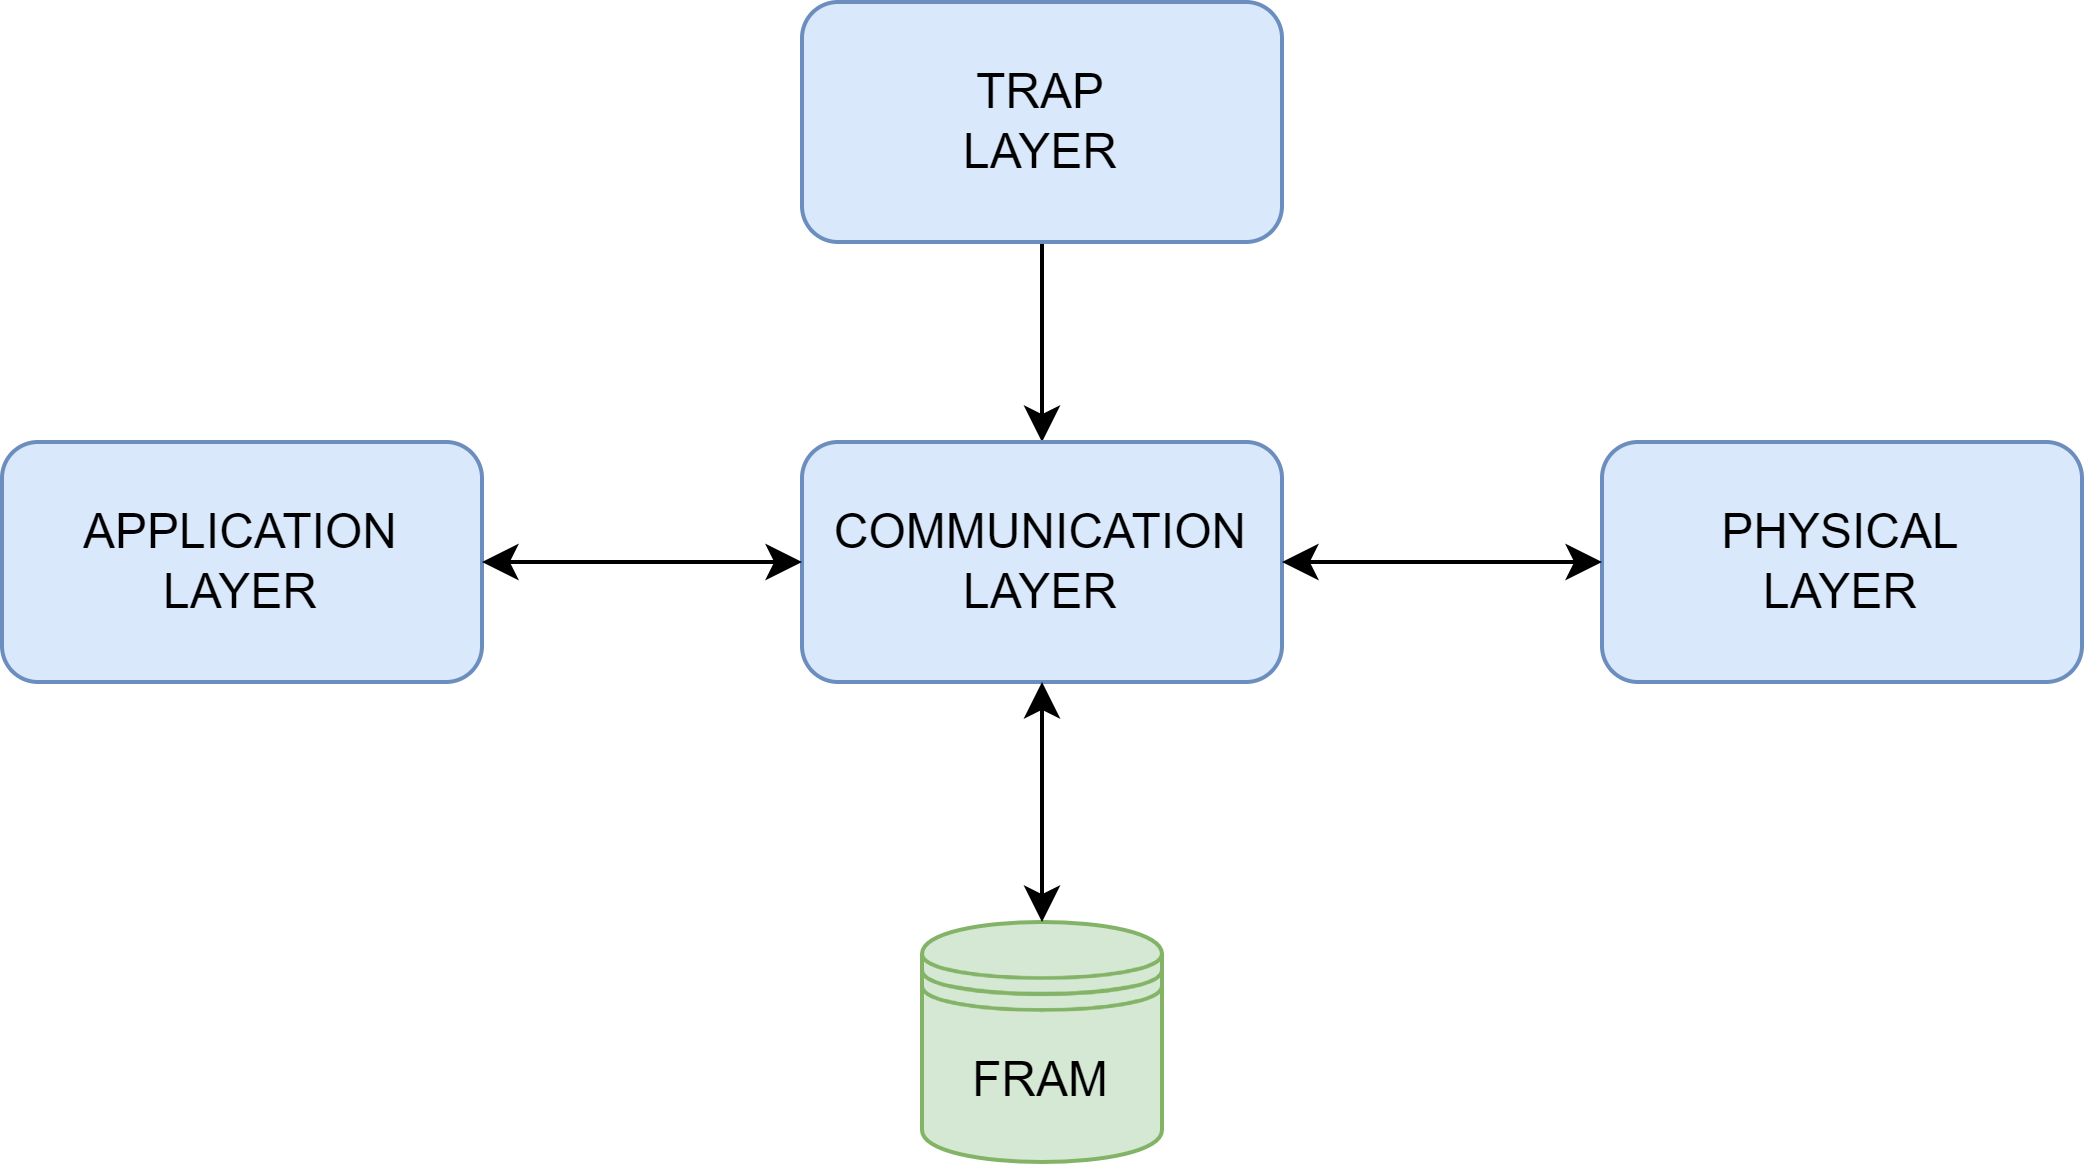
\psfig{file=Images/systemArchitecture.png,width=0.8\textwidth}}
    \caption{\footnotesize \centering System architecture diagram: Application Layer, TRAP Layer, Communication Layer and Physical Layer}
    \label{fig:SystemArchitectureDiagram}
  \end{figure}
 \subsection{Application Layer}
This section contains the abstractions that allow the programmer to develop an application using the implemented network stack.\\
The functions exposed by the Communication Layer allow high-level data sending and receiving. All memory management, transmitting, and receiving are executed automatically by the stack.\\
An example of an Application Layer, in pseudo code, might be as described below:\\
\begin{lstlisting}
....
while (1)
{
    value = collectDataFromSensor();
    destinationNode = 1;
    dataProduced(value, destinationNode);
    dataSend();
}
....
\end{lstlisting}
\subsection{TRAP Layer}
The Trap Layer is the layer that implements the TRAP protocol.\\
It is based on the use of timers for repetitive burst sending, OOK modulation, and sending node identification.\\
The bursts contain encoding of the energy level of the sending node. Each neighboring node in the network sends its energy level at fixed intervals.\\
Recognition of the sending node is accomplished by an analysis of the burst sending frequency.\\
\subsection{Communication Layer}
Communication Layer is the part of the system responsible for sending and receiving data from the Physical Layer and the Application Layer.\\
The Communication Layer does much more than what has just been explained: it is responsible for managing the data within non-volatile memory (FRAM \cite{FRAM})  so it is the heart of the system.\\
FRAM management consists of saving and retrieving data; this mechanism helps limit packet losses during power failures.\\
\subsection{Physical Layer}
The Physical Layer is the layer responsible for actually sending and receiving packets.\\
It is easily replaceable and allows the use of different transmission technologies such as backscatter communication or visible-light communication.\\
In this implementation, the choice fell on the use of a UART communication.\\
A whole chapter will not be devoted to explaining the layer as it is of little significance to the implementation. It will be mentioned in the evaluation section to give context to the tests performed.
  
\newpage





      \chapter{System Implementation}
\label{cha:communicationStack}
The purpose of this chapter is to show how the complexity of the system was hidden from the Application Layer through the use of methods exposed by the TRAP and Communication Layers.
\section{TRAP Layer}
\label{sec:TRAPLayer}
The TRAP Layer is the layer that implements the TRAP protocol.\\
The purpose of this layer is to allow reliable communication between nodes by reducing power failure allowing transmission only under certain conditions. Specifically, communication can only occur if the sending node and the receiving node have sufficient energy levels to send and receive the packet \cite{9733918}.\\
As the protocol is designed, this layer is based on the repeated sending at fixed intervals in time of a series of pulses that encode the node's energy level. On the other hand, the layer must receive the energy levels of neighboring nodes within the network and correctly associate them, through sending frequency recognition, with the transmitting node. For this reason, the basic implementation idea exploits timers on the MSP430 board to perform repetitive burst sending (series of pulses, varying in length depending on the energy accumulated by the node) and externals GPIO interrupts generation to handle incoming bursts.\\
To correctly associate the incoming burst with the sending node, the adopted solution is to have a timer count from the beginning of the reception and stop it at the end of the reception, then calculate the sending frequency.\\
Based on the energy level of the node and the energy level received from other nodes, the layer decides whether or not transmission can be made to and from the node.\\
\begin{figure}[H]
\centerline{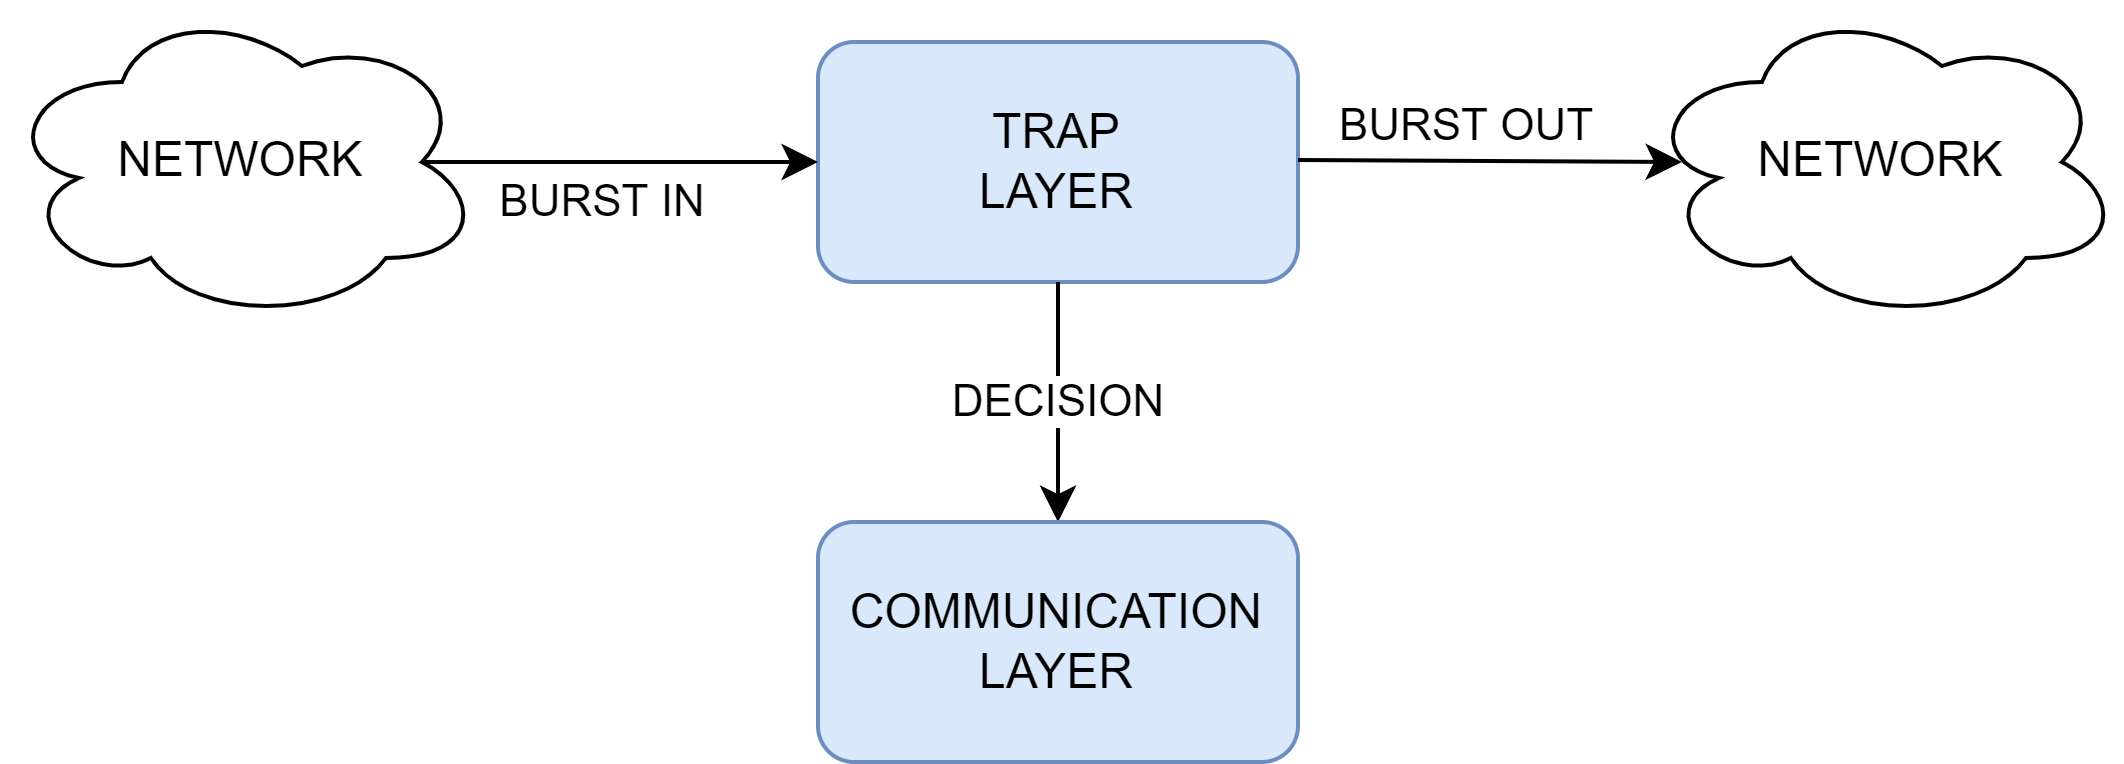
\psfig{file=Images/TRAPLayerDetails.png,width=0.7\textwidth}}
\caption{\footnotesize \centering TRAP Layer representation}
\label{fig:TRAPLayerDiagram}
\end{figure}
This Layer exposes a single function to check whether the energy level of the sending node and the receiving node is sufficient to complete the transmission. The return value of the method is 1 if sending is possible, and 0 otherwise.
\section{Communication Layer}
\label{sec:CommunicationLayer}
This section of the system contains the infrastructure needed to limit the loss of data and consequently the waste of energy following a power failure. More specifically: saving data to non-volatile memory, restoring data from non-volatile memory, sending data to the Physical Layer, sending data to the Application Layer, and checking data validity in case of expired packets.\\
Control over packet expiration is included within the sending of data to the Physical Layer and the Application Layer. For this reason, it will be discussed in those sections and not in a dedicated part.\\
Before analyzing the implementation choices in detail, it is convenient to indicate the package structure used by the layer for processing.
\subsection{Packet Structure}
\label{sec:PacketStruct}
 The package is defined as follows:
\begin{table}[H]
\begin{center}
\begin{tabular}{ |c| c| c| c| c| c| c| c|}
 NODEID & DATA0 & DATA1 & DATA2 & DATA3 & CRC0 & CRC1 & TIMESTAMP\\ 
\end{tabular}
\caption{\label{tab:Packet format}Package structure, 64bit}
\end{center}
\end{table}
The packet consists of 8 byte-sized fields. Specifically, the first field indicates the producing node, the next four the data produced, then we find two CRC fields used to detect any errors in transmission, while the last field indicates the production timestamp of the packet.\\
It is important to note that the fields are byte-sized, this allows atomic operations in memory.
\subsection{Data Saving From Application Layer (Data saving TX)}
\label{sec:CommLayer1}
The Application Layer calls the producedData() method passing as arguments four bytes of data and one byte indicating the message recipient node identifier.\\
After the data reception, the Communication Layer begins saving the data in non-volatile memory.\\ 
Data saving takes place in structures containing the message fields. 
\begin{lstlisting}%
[caption={Structure containing the package fields and two supporting fields for managing the package in memory},label=lst:struttura,frame=trbl]
typedef struct storedData
{
    unsigned char nodeNumber, data0, data1, data2, data3, CRC0, CRC1, timeStamp, saved, nodeRX;
} storedData;
\end{lstlisting}
These structures are arranged in a circular buffer (Buffer TX). 
For this purpose, it is important to keep track of the last location written to the buffer in case of power failure. 
This is needed to avoid inadvertent overwriting of data. 
To do this it is necessary to save in non-volatile memory a field that will serve as a pointer.\\
The four data passed to the function are saved directly, byte by byte, in non-volatile memory along with the producer node value (the latter value is already known to the Communication Layer and does not need to be passed by the Application Layer).\\
Next, the Communication Layer proceeds to calculate the CRC16 value of the four bytes of data passed by the Application Layer. The resulting two bytes are saved in non-volatile memory too.\\
At this point, the packet time stamp, and the recipient node identifier are added.\\
The packet will be confirmed as saved by setting a control byte to 1 and incrementing the buffer pointer.\\
Finite state machine of data saving from Application Layer is presented in Figure \ref{fig:FSMSAVETX}.\\
If no power failure is encountered during saving, the package is saved correctly and ready to be sent when requested by the application layer.\\
On the contrary, any power failure before the pointer increment would render the data unusable and would be overwritten at the next save request by the Application Layer.\\
\begin{figure}[H]
\centerline{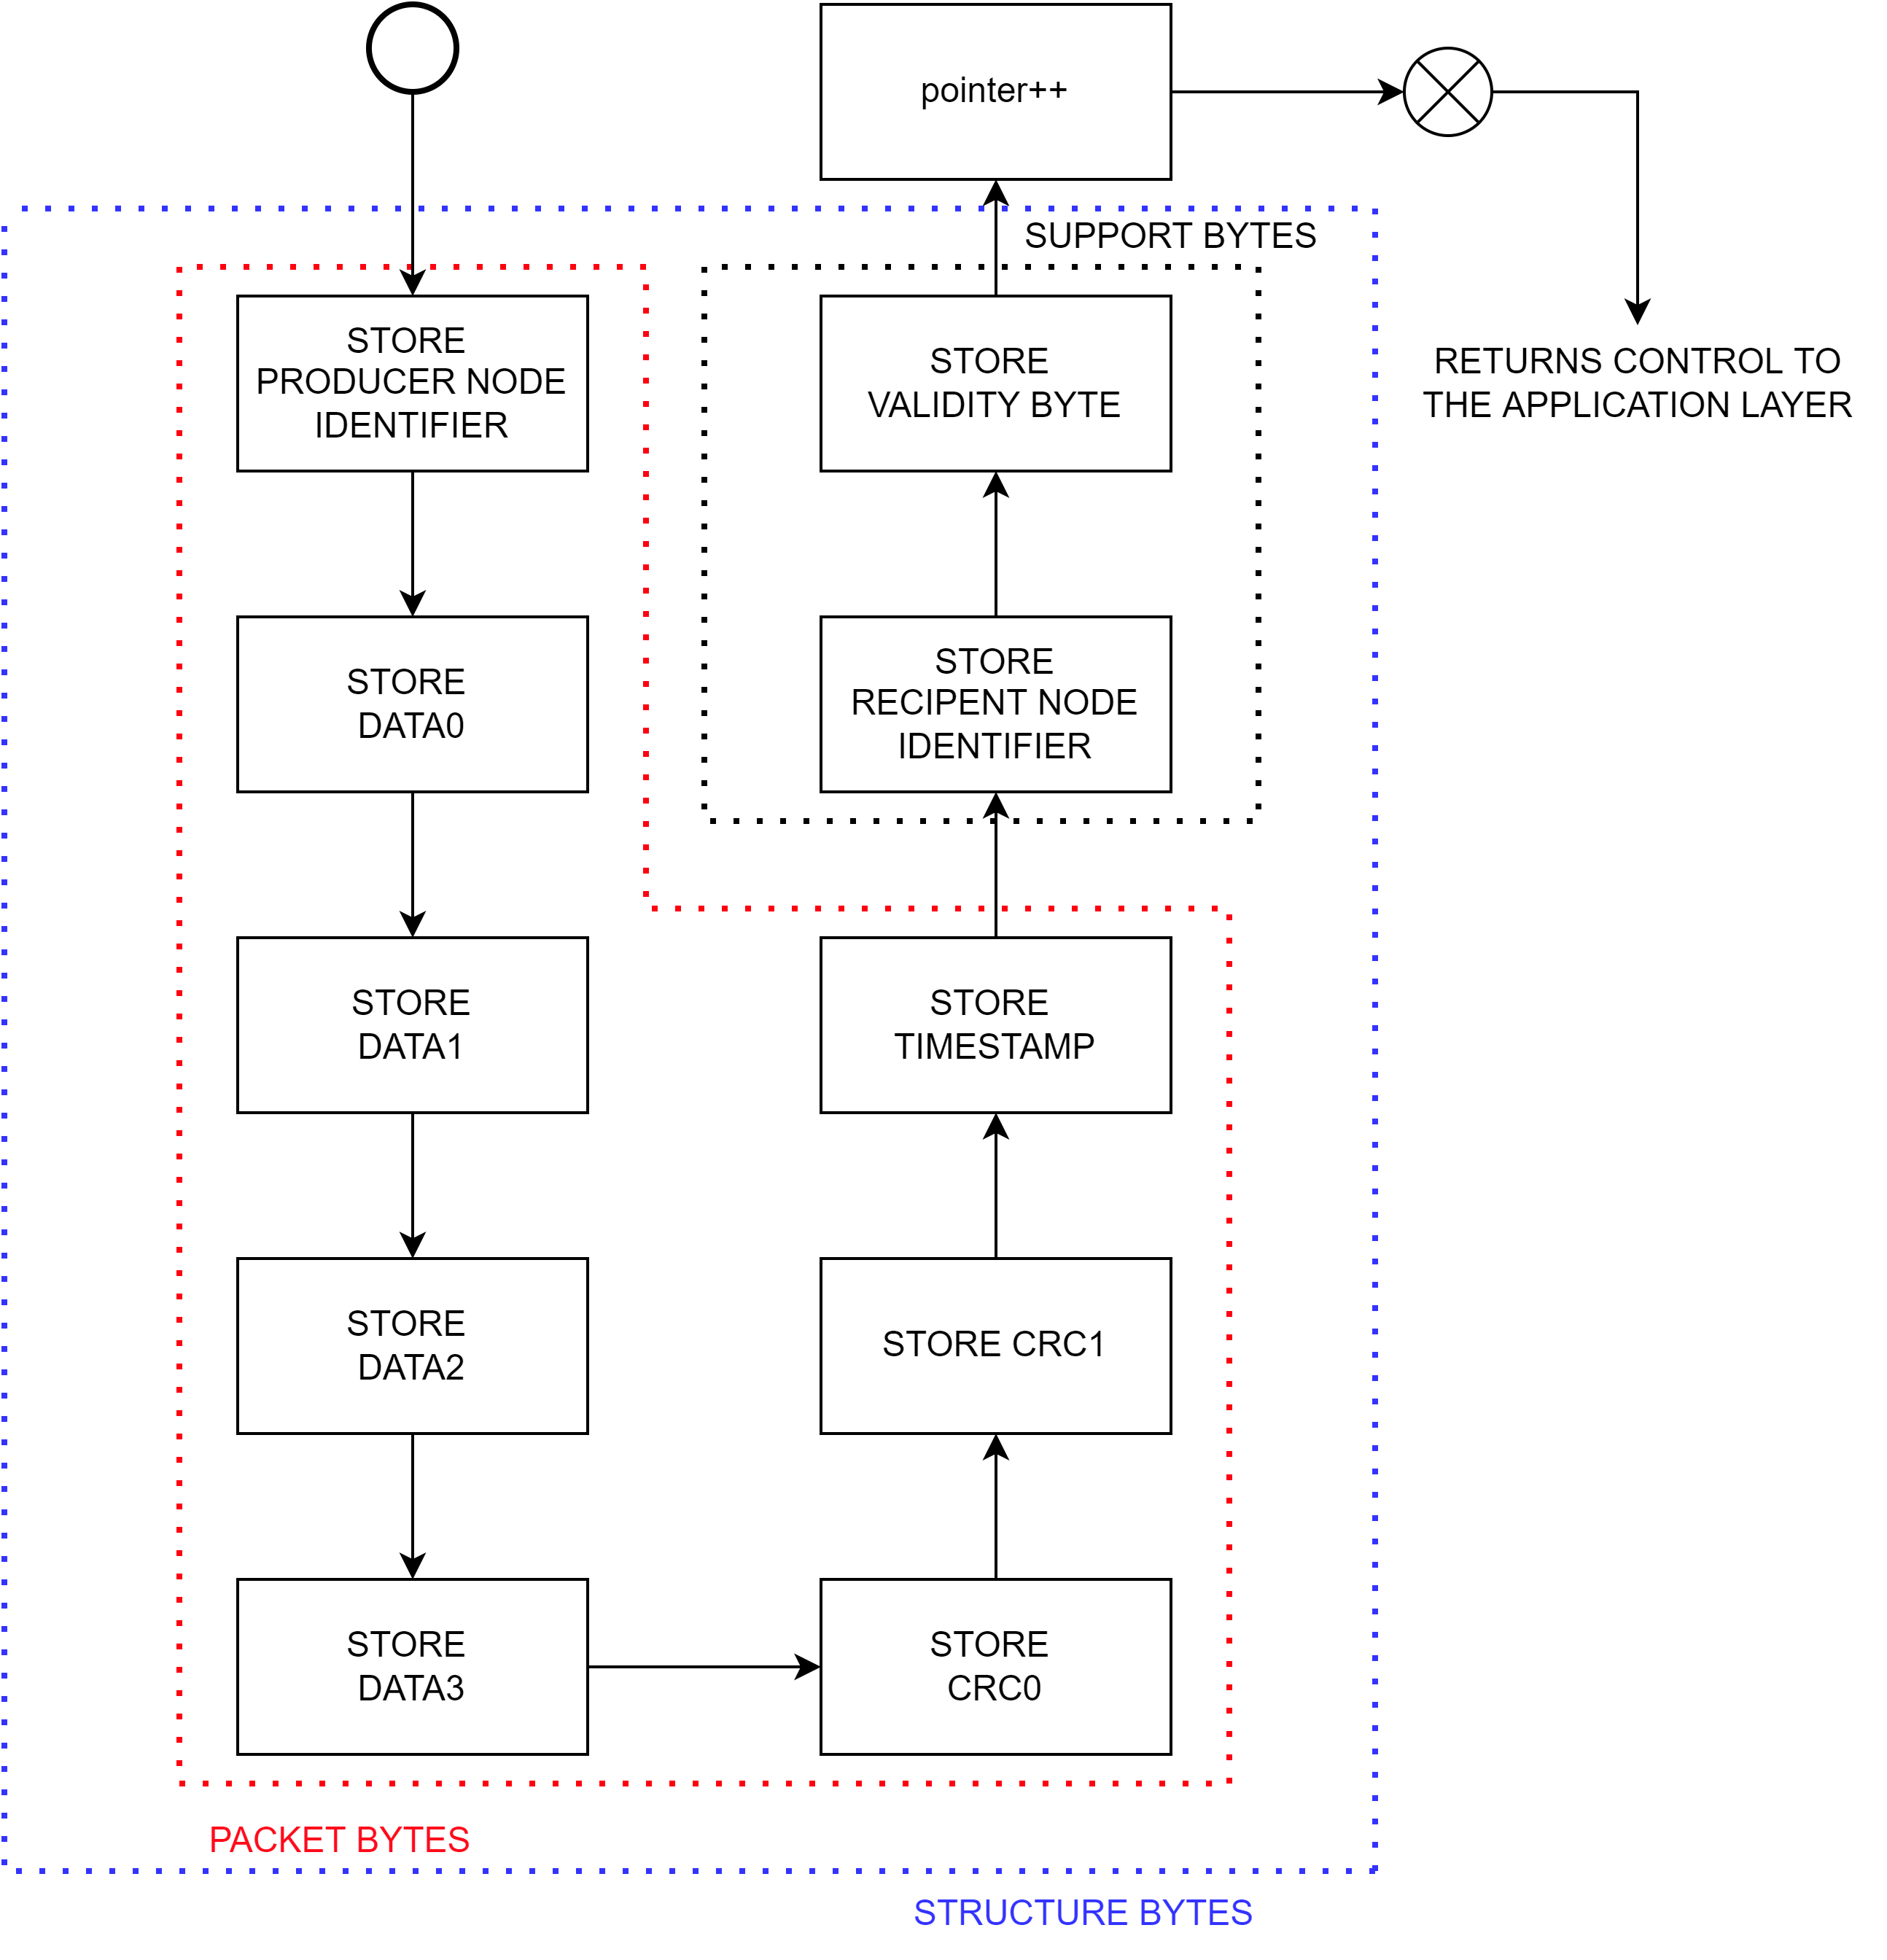
\psfig{file=Images/SaveTX-FSM.png,width=0.8\textwidth}}
\caption{\footnotesize \centering Finite state machine related to package building and saving (pointer: writePointer)}
\label{fig:FSMSAVETX}
\end{figure}
\subsection{Data Sending To Physical Layer (Data TX)}
\label{sec:CommLayer2}
To send the data produced, the Application Layer must call the dataSend() method without passing arguments.\\
When this method is invoked, the Communication Layer chooses the packet stored in non-volatile memory to send and forwards it to the Physical Layer.\\
The selection of the packet to be sent is the most relevant section of this method.
The packets to be sent are stored in a circular buffer, so you have to keep track of the packet by a pointer stored in non-volatile memory. The logic is the same as shown in the data saving. The pointer is incremented only when the operation is completed and the validity byte is reset to 0. This is important in case of power failure, if the control byte was reset before the sending was completed, the packet would be marked as sent when in fact it was not.\\
The data is considered valid only if the control byte (set during packet saving) is set to 1.\\
Choosing the packet to be sent only with the pointer, however, is not the best solution. 
In fact, before each send, the canSendTRAP() method of the TRAP layer is called to check whether it can be transmitted to the recipient node.\\
If a recipient node A shuts down and the buffer contains messages for nodes A, B and C in that order, the insufficient energy level of A blocks the messages for B and C. In order to avoid that, the node sends the next packet in the buffer (i.e. the one for B), if possible, otherwise it tries with the next again and so on.\\
The solution adopted involves a priority check on the packet indicated by the pointer. If it cannot be sent, checks are made on subsequent packets until a sendable packet is reached or the entire buffer is scrolled (Figure \ref{fig:FSMSENDTX}).
\begin{figure}[H]
\centerline{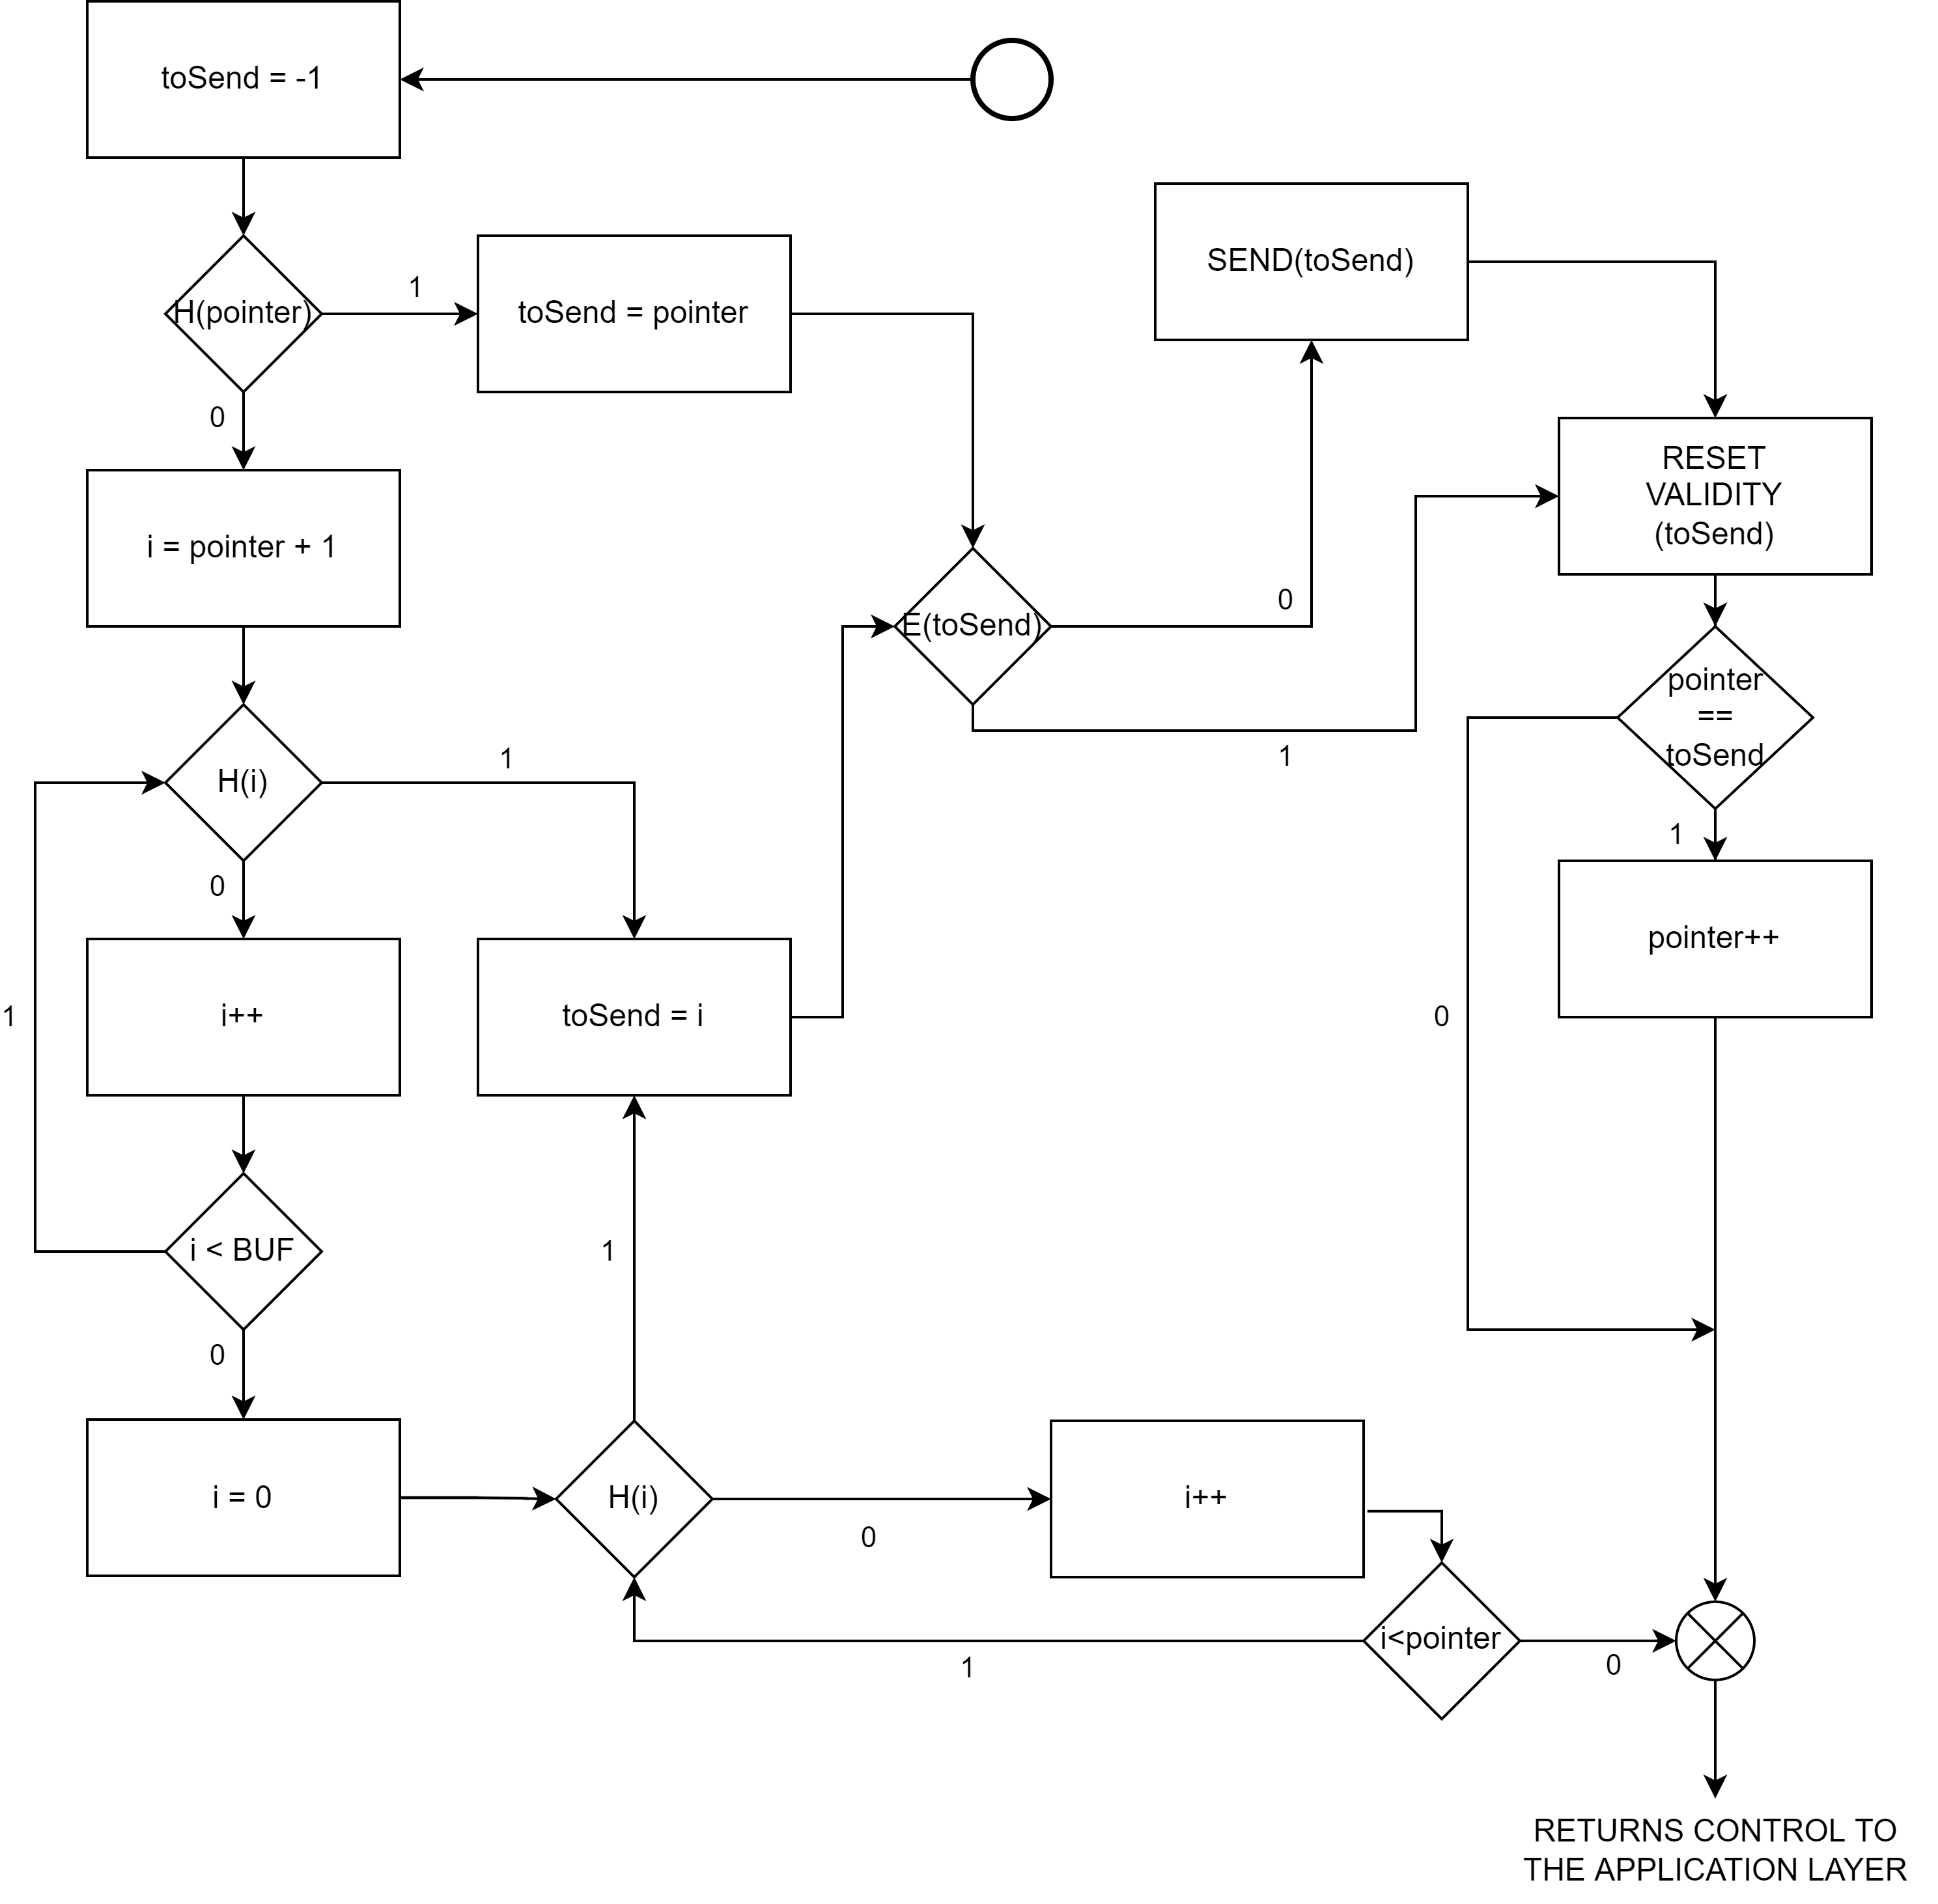
\psfig{file=Images/sendTX-FSM.png,width=0.75\textwidth}}
\caption{\footnotesize \centering Finite state machine related to package selection and sending (H(x): (checkValidity(x) \&\& canSendTRAP(x)), E(x): expiration(x), pointer: sendPointer, BUF: TX Buffer size)}
\label{fig:FSMSENDTX}
\end{figure}
\subsection{Data Saving From Physical Layer (Data saving RX)}
\label{sec:CommLayer3}
Saving data received from the Physical Layer is done in much the same way as presented for saving data from the Application Layer. Again, data saving occurs in structures containing message fields arranged within a circular buffer (Buffer RX). This requires a pointer to keep track of the last position written.\\
The Physical Layer notifies by triggering an interrupt the Communication Layer at the end of data reception.\\
The Communication Layer checks whether the received packet consists of 8 bytes. If the received packet is complete, the Communication Layer checks for errors via a CRC16 module. If no errors are detected the packet validity byte is set to 1 and the receive buffer pointer is incremented. The pointer, as explained earlier, is not incremented before packet acknowledgment because in case of power failure it could lead to marking inconsistent packets as good.
\begin{figure}[H]
\centerline{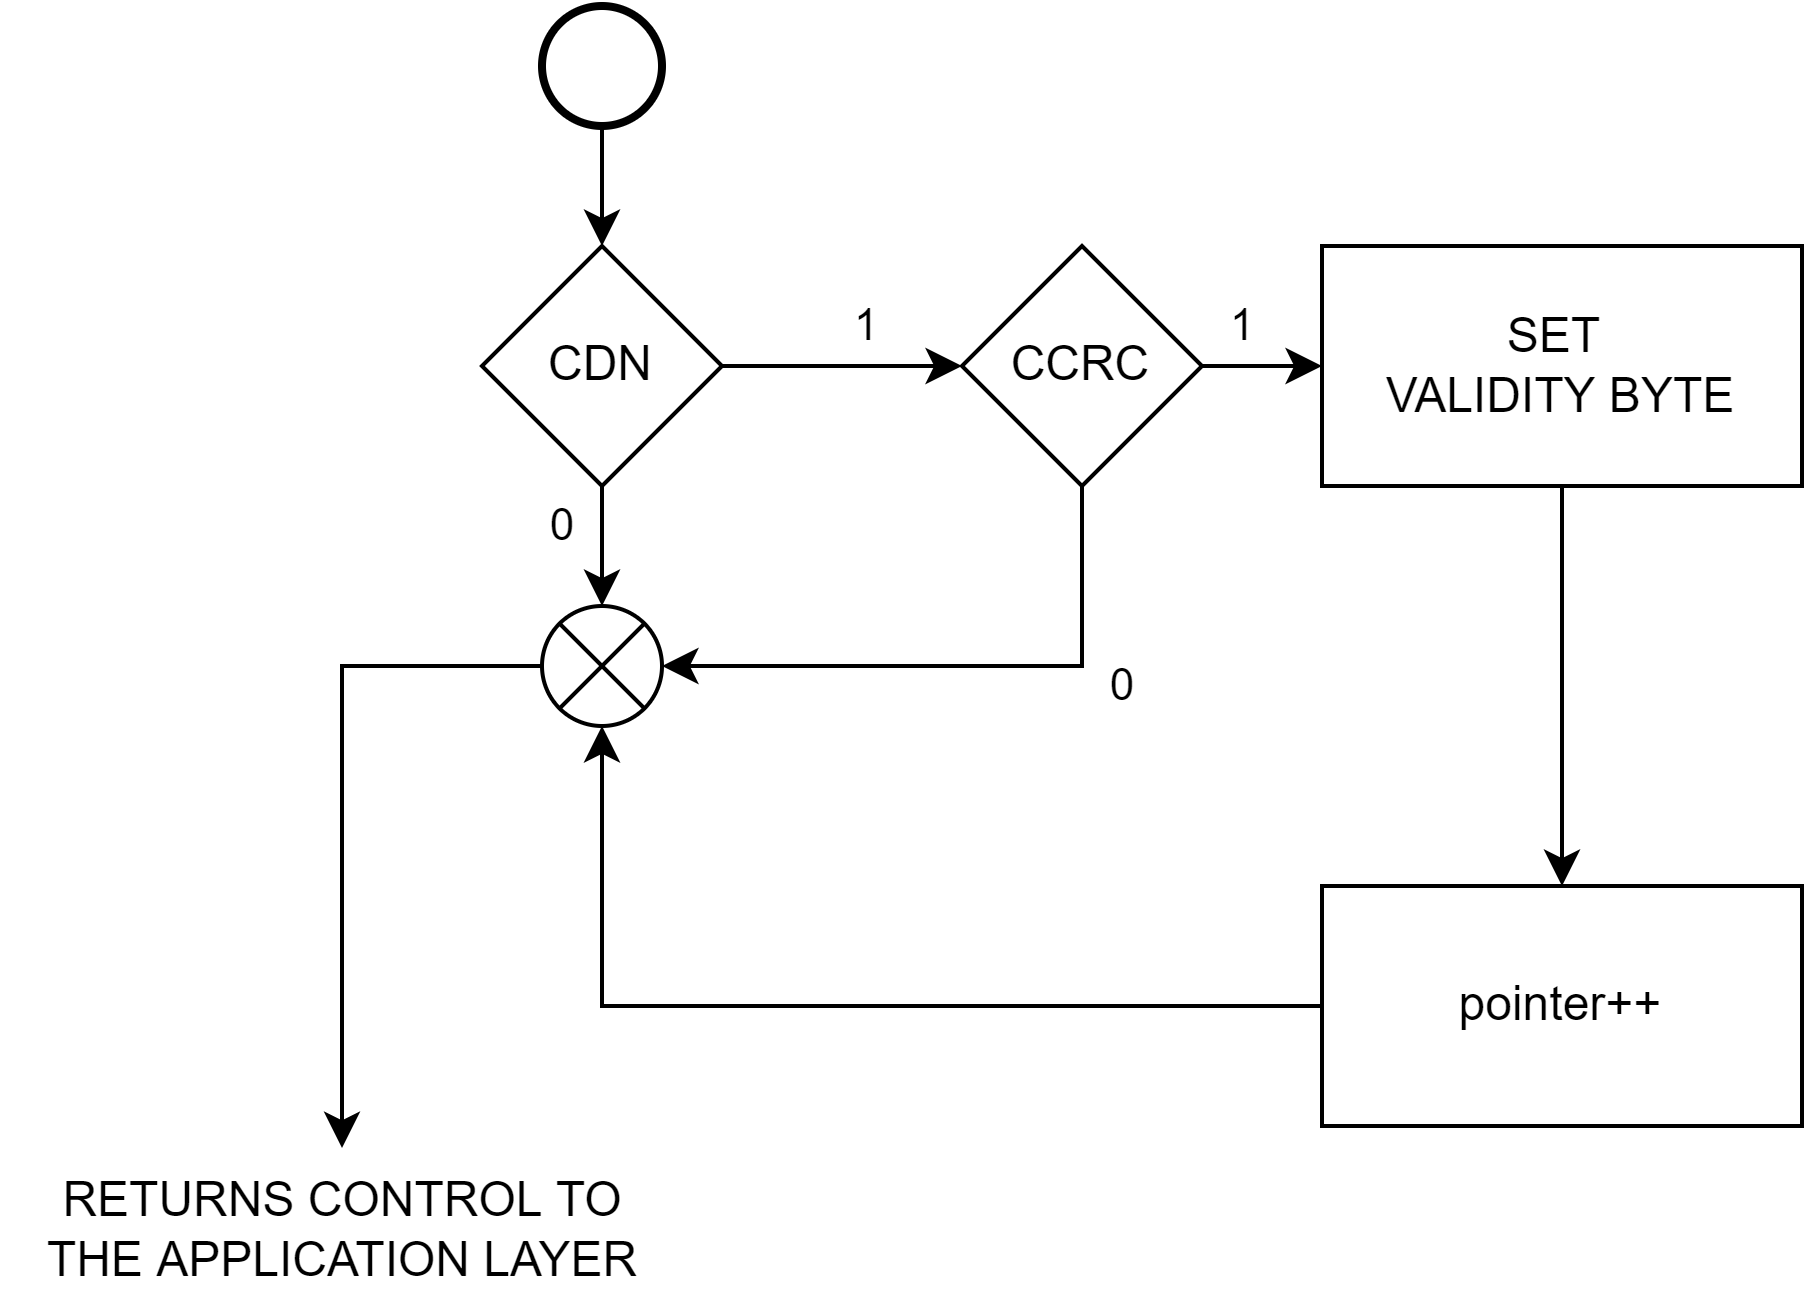
\psfig{file=Images/saveRX-FSM.png,width=0.65\textwidth}}
\caption{\footnotesize \centering Finite state machine related to Data saving RX (CDN: checkDataNumber(), CCRC: checkCRC())}
\label{fig:FSMSAVERX}
\end{figure}
\subsection{Data Sending To Application Layer (Data RX)}
\label{sec:CommLayer4}
The forwarding of packets from the Communication Layer to the Application Layer is done by the call of the getData() function.\\
The Application Layer receives a structure containing the first available packet saved in memory if present, a packet initialized to zero otherwise.\\
When the getData() function is called, the Communication Layer scrolls through all the packets saved in the RX buffer to delete the expired ones.\\
Thereafter, the packet choice is made similarly to what was seen for sending to the Physical Layer. The difference, concerning what was presented earlier, is related to the TRAP check that does not have to be performed.\\
For the location of the packet to be transmitted within the buffer, a pointer is saved in non-volatile memory. This pointer will be incremented only after the validity byte of the structure containing the data is reset.
\begin{figure}[H]
\centerline{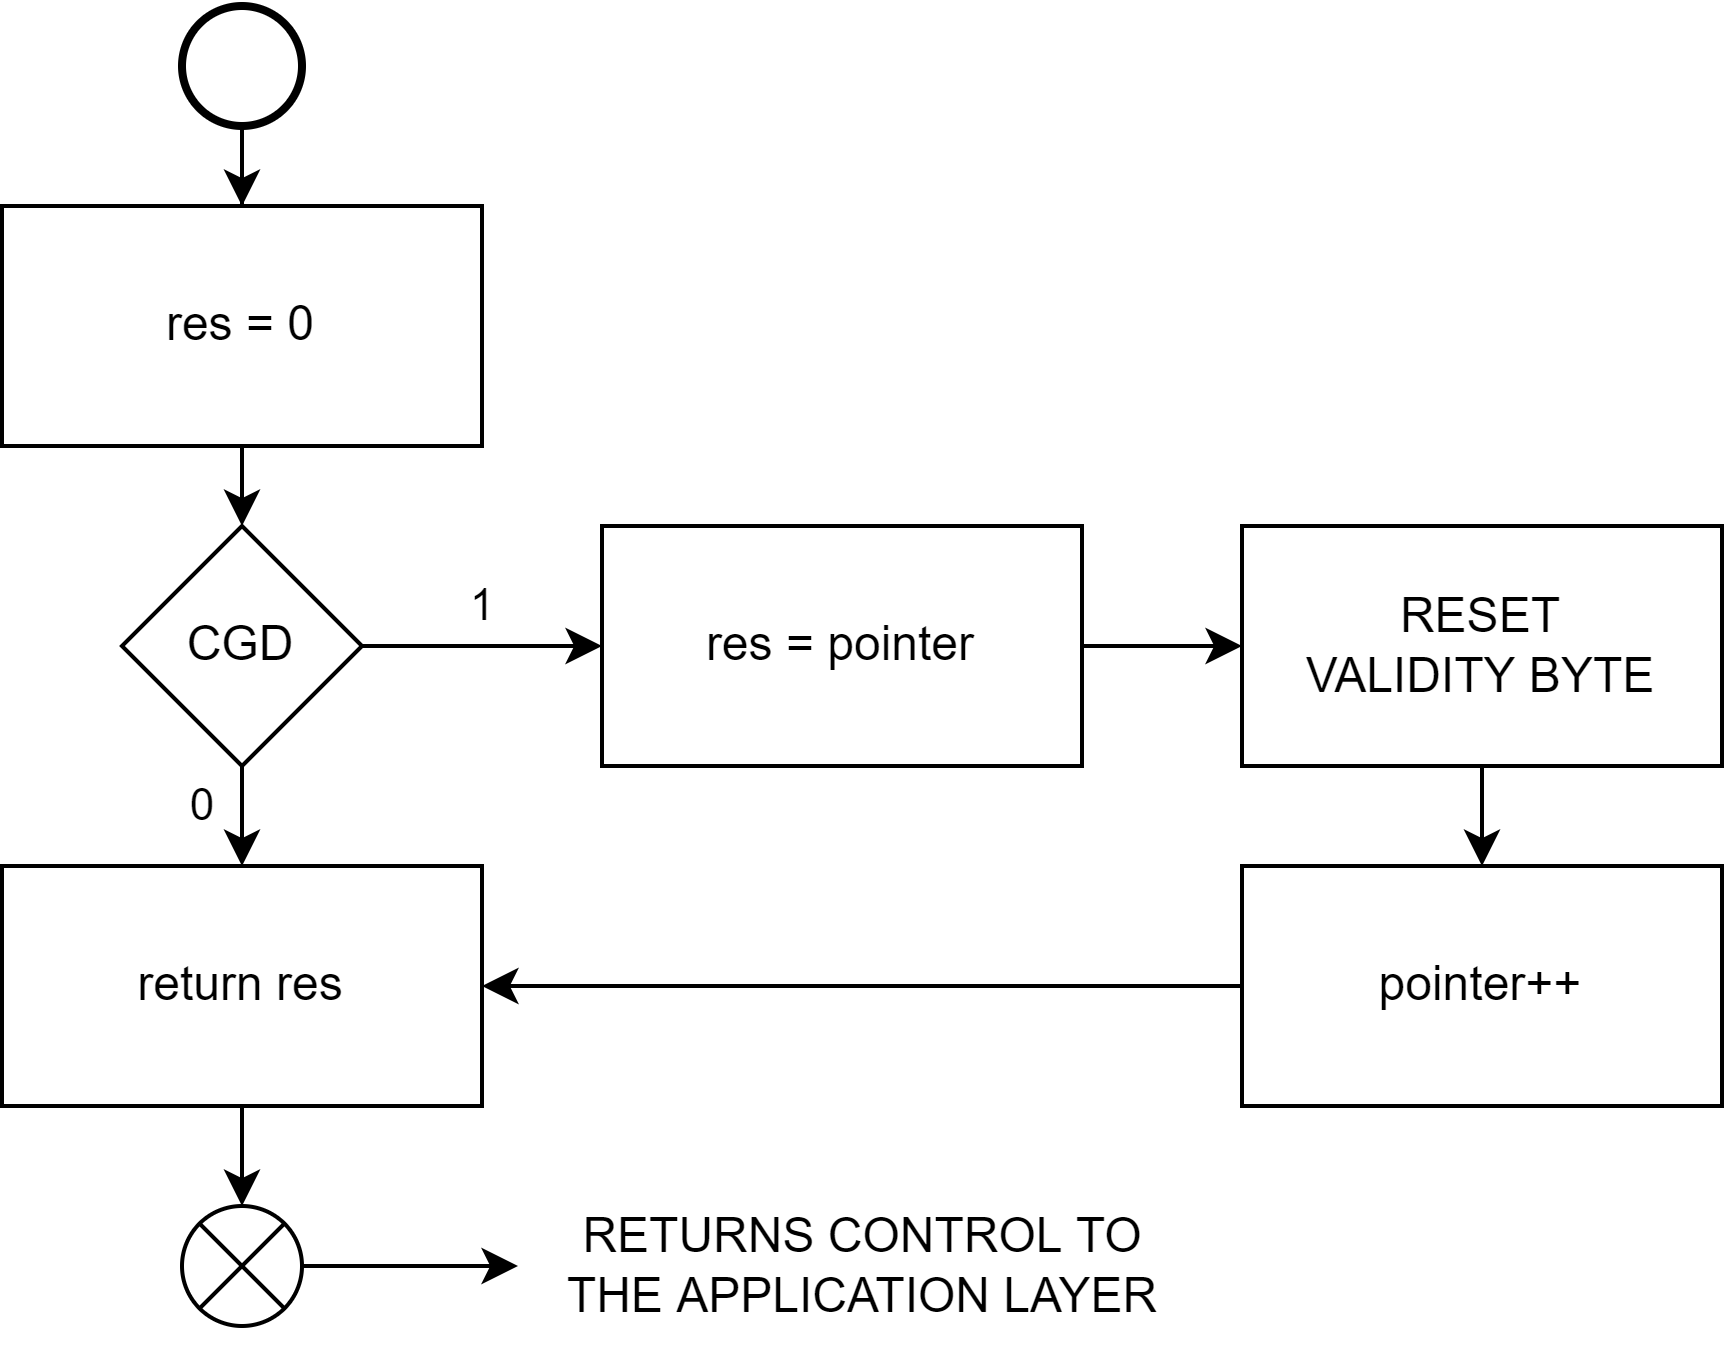
\psfig{file=Images/dataGet.png,width=0.65\textwidth}}
\caption{\footnotesize \centering Finite state machine related to getData() function (CGD: canGetData())}
\label{fig:DATAGET}
\end{figure}
\section{Power Failure Resistance}
\label{sec:PowerFailureResistance}
Since power failure resilience is the novelty of this thesis, it is worth spending a few words explaining what happens in case of power failure during normal system operation such as during sending data from the Application Layer to the Communication Layer, forwarding data from the Communication Layer to the Physical Layer for sending to the network, receiving data from the network to the Physical Layer and forwarding to Communication Layer, and during data sending from the Communication Layer to the Application Layer.\\
\subsection{From The Application Layer To The Communication Layer}
In this case, we have several possibilities:
\begin{enumerate}
\item Power failure occurs before the packet is acknowledged through the validity byte set
\item Power failure occurs immediately after the packet validity byte set but before the pointer increment that signals the location to be written to the buffer
\item Power failure occurs after the packet validity byte set and after the pointer increment that signals the location to be written to the buffer (just before the return from the function to the Application Layer)
\end{enumerate}
In the first scenario, the partially saved packet will be overwritten at the next data pass by the Application Layer. This is the worst situation because the data cannot be sent. The energy used to produce it has been wasted.\\\\
In the second scenario, the situation is slightly better than shown above. The packet will, again, be overwritten on the next pass of data by the Application Layer. However, having the validity byte set to 1 makes it possible to send it if it is not overwritten first. This operation could be useful when the Application Layer produces less data than can be sent as it would still allow the packet to be sent. The power produced to produce the data is considered lost only if the packet is overwritten.\\\\
In the third situation, the power failure is of no consequence since the packet is marked as saved correctly and thus can be sent following the Application Layer request. Similarly, the pointer to the buffer location is incremented, consequently, a new data save call by the Application Layer would not overwrite the packet since the next location in the buffer would be written.\\
\subsection{From The Communication Layer To the Physical Layer}
A power failure during data transfer from the Communication Layer to the Physical Layer is a remote possibility; in fact, this transfer is either authorized or denied by the TRAP protocol.\\
However, developing a system that relies only on the TRAP protocol and has no persistent management of packets to be sent does not seem like a good solution.\\
Therefore, we can consider and show how packets are handled in case of power failure during sending from the Communication Layer to the Physical Layer. It should be remembered that sending data from the Communication Layer to the Physical Layer occurs only when the TRAP protocol responds affirmatively to the possibility of sending the packet to a particular node. Data sent to the Physical Layer is immediately forwarded to the recipient node.\\
In this case, we have several possibilities:
\begin{enumerate}
\item Power failure occurs before the packet validity byte is reset
\item Power failure occurs after the reset of the packet validity byte
\end{enumerate}
In the first case, the packet is not marked as sent since the validity byte is not changed. The packet will be resent when possible. The power used to send part of the packet is lost.\\\\
In the second case, the validity byte is reset, and then a power failure occurs. The way the stack is implemented, if the validity byte is set to zero, the packet can no longer be sent and will be overwritten in subsequent saves by the Application Layer. However, resetting the byte to zero implies sending the data completely. In this situation, the pointer relative to the location in the buffer of the packet to be sent is not incremented; again, this is not a problem because the Communication Layer performs checks on the validity of the packet before forwarding it to the Physical Layer.
\subsection{From The Network To The Physical Layer}
A possible power failure during the reception of data from the Physical Layer to the Communication Layer is a situation that would be unlikely to occur; in fact, even this transmission takes place under the control of the TRAP protocol.\\
If this happens, however, the system is designed to discard the packet if it has not been marked confirmed with the validity byte set.
Specifically, the Physical Layer starts a timer upon receipt of the first piece of data. This timer is restarted with each new reception.\\
At the moment when the timer generates an interrupt, and thus no data has been received for a given time interval, the Communication Layer is called to perform a check on the amount of data that has arrived. This check is used to verify that all 64 bits of the packet have been received.\\
If a power failure occurs before the packet validity byte is set by the Communication Layer, the data is discarded and is not sent, when requested, to the Application Layer. In this case, the energy expended in receiving and transmitting the packet is wasted.
\subsection{From The Communication Layer To The Application Layer}
To receive the packet from the Communication Layer, the Application Layer must call a function that returns a packet saved in the RX buffer of the Communication Layer.\\ 
If the power failure occurs after the Communication Layer resets the packet validity byte, the packet is lost. This happens in the case where the power failure occurs during the return from the function to the Application Layer.\\
In the case, on the other hand, where the power failure occurs before the validity byte reset, the packet can be requested again at the Communication Layer since it will still be valid.
\newpage
      %\chapter{TRAP Layer}
\label{cha:TRAP Layer}
The TRAP Layer, as mentioned in previous chapters, is the layer that implements the TRAP protocol. The purpose of this layer is to allow reliable communication between nodes by reducing power failure to the limit and thus allowing transmission only under certain conditions. Specifically, communication can only occur if the sending node and the receiving node have sufficient energy levels to send and receive the packet \cite{9733918}.\\

\section{Implementation idea}
\label{sec:Implementation idea}
As the protocol is designed, this layer is based on the repeated sending at fixed intervals in time of a series of pulses that encode the node's energy level. On the other hand, the layer must receive the energy levels of neighboring nodes within the network and correctly associate them, through sending frequency recognition, with the transmitting node. For this reason, the basic implementation idea exploits timers on the MSP430 board to perform repetitive burst sending (series of pulses, varying in length depending on the energy accumulated by the node) and interrupt generation to handle incoming bursts.\\
To correctly associate the incoming burst with the sending node, one possible solution is to have a timer count from the beginning of the reception and stop it at the end of the reception, then, with an easy mathematical calculation, obtain the sending frequency.\\
Based on the energy level of the node and the energy level received from other nodes, the layer decides whether or not transmission can be made to and from the node.

\section{Layer diagram}
\label{sec:Layer diagram}
The figure below represents the TRAP Layer diagram. The input burst, output burst, and outward exposure of evaluation can be observed.\\
  \begin{figure}[h!]
    \centerline{\psfig{file=Images/TRAPLayer.png,width=0.5\textwidth}}
    \caption{\footnotesize \centering TRAP Layer representation}
    \label{fig:TRAPLayerDiagram}
  \end{figure}
 
In this implementation, the node energy is simulated within the node. In a real application, the TRAP Layer would be connected to the poles of a capacitor (or a battery) to obtain the current energy level.

\section{Real implementation of the layer}
\label{sec:Real implementation of the layer}
Following the implementation idea given above, it is possible to discuss the actual implementation of the layer.
In particular, the operation is based on the use of four timers. Timers are realized by registers that automatically increment their value with the frequency at which they are configured. On the MSP430 board, timers have several modes of operation: the "UP mode" will be considered in which the timer counts up to a preset value, generates an interrupt, and resets its value to zero restarting counting again if not stopped.\\
  \begin{figure}[h!]
    \centerline{\psfig{file=Images/TimerMode.png,width=0.5\textwidth}}
    \caption{\footnotesize \centering "UP Mode" timer diagram}
    \label{fig:TimerMode}
  \end{figure}
For timer configuration the reference is the site of Texas Instruments, the manufacturer of the board.\\
Timers used for this layer are:
\begin{itemize}
  \item Timer A1 at 250Hz for Burst repetition
  \item Timer A2 at 1MHz to calculate the frequency in reception
  \item Timer A3 at 32kHz for burst timeout and avoid glitches
  \item Timer B0 at 1MHz to create the OOK modulation
\end{itemize}
To analyze the operation of the system, we divide it conceptually into transmitting side (TX) and receiving side (RX).

\subsection{TX side of TRAP Layer}
For proper operation of this part of the Layer, we will use timers A1 and B0 set as above and both in "UP mode". Remember that in this mode the timer will count until the value within the CCRx (capture/compare registers) is reached and then generate an interrupt. The CCR0 register of timer A1 is set to 250 so that there is a one-second delay between one burst and the next, energy level sending frequency is so set to 1 Hz.\\
In the TRAP Layer, there is an internal function that receives the energy level of the node and encodes it in the form of bursts to obtain the number of pulses to be sent to communicate the correct available power.\\
\begin{lstlisting}
//CCR0 register setting of timer B0
TB0CCR0 = (1000 / (OOK_NODE * 2));
\end{lstlisting}
This setting allows the burst sending pin to be toggled at a frequency equal to OOK. Remember that each node has an OOK frequency chosen and set in advance to distinguish it from other nodes in the network. Multiplier 2, in the formula, is used to have the correct number of rising and falling edges; in fact, each time timer B0 generates an interrupt the signal on the burst send pin will be inverted and to have, for example, 64 pulses the signal must be inverted 128 times.\\
  \begin{figure}[H]
    \centerline{\psfig{file=Images/TRAPLayerTimer.png,width=0.45\textwidth}}
    \caption{\footnotesize \centering Block diagram of TRAP Layer TX}
    \label{fig:TRAPLayerTimer}
  \end{figure}
  
\subsection{RX side of TRAP Layer}
This side of the layer deals with the reception of bursts and the correct recognition of the transmitting node.\\
Timers A2 in "Continuous Mode" and A3 in "UP Mode" were used to implement the reception side. Timer A2 is used as a counter to calculate the frequency of receiving pulses. Timer A3 is used to figure out when the burst is finished. When timer A3 end, begin operations to assign the correct received energy level to the network node that transmitted it.\\
When the first pulse is received on the GPIO pin dedicated to receiving the burst, timer A2 is activated, and timer A3 is restarted each time a new pulse is received. The latter timer is set to count 15 times at a rate of 32kHz; if no further pulses were received in this time interval, it is reasonable to assume that the burst is over. Timer A2 can be stopped, the counted value read, and the evaluations made to decode the energy level and associate it with the correct node.\\
  \begin{figure}[H]
    \centerline{\psfig{file=Images/TRAPLayerRX.png,width=0.65\textwidth}}
    \caption{\footnotesize \centering Diagram of TRAP Layer RX}
    \label{fig:TRAPLayerRX}
  \end{figure}
\begin{lstlisting}
//Basic implementation idea for the interrupt related to the GPIO pin of the incoming burst
if (count == 0)
    {
        NODE_ID_CR = TASSEL_2 + MC_2 + NODE_IDENTIFICATION_DIVIDER; //Start timer A2
        BURST_TIMEOUT_CR = TASSEL_1 + MC_1 + ID_3; //Start timer A3
    }
    count++;
    BURST_TIMEOUT_EV = 0; //Stop timer A3
    BURST_TIMEOUT_EV = TIMEOUT; //Restart timer A3
\end{lstlisting}

\begin{lstlisting}
//Basic implementation idea for the interrupt related to the timeout timer (Timer A3)
if (count > (64 - BURST_GUARD))
    {
        frequency = ((float) NODE_IDENTIFICATION_SPEED * (float) count) / 
        ((float) timerValue);
    }
\end{lstlisting}

  
\newpage





      %\chapter{Communication Layer}
\label{cha:Communication Layer}
The Communication Layer is the intermediary between the Application Layer and the Physical Layer. In this layer, data is received from the physical layer, manipulated, stored in FRAM memory, and then sent to the application layer when requested. Symmetrically, the layer receives data from the Application Layer, structures the packet to be sent, and forwards it to the Physical Layer.

\section{Implementation idea}
\label{sec:Implementation idea Comm}
The relevant part of this layer is the storage of received data in the FRAM memory and consequently the proper management of reading and writing from and to the memory.
The basic idea for the implementation of this layer is to use circular buffers with FIFO (first in, first out) logic. In this way is possible to have different sections of memory for input data (RX) and output data (TX) and the possibility to overwrite old data.


\section{Layer diagram}
\label{sec:Layer diagram Comm}
This section reinforces, through the use of a diagram, the connection between the layer and the FRAM. 
  \begin{figure}[H]
    \centerline{\psfig{file=Images/CommunicationLayerDiagram.png,width=0.5\textwidth}}
    \caption{\footnotesize \centering Block diagram of Communication Layer}
    \label{fig:CommunicationLayerDiagram}
  \end{figure}
The communication layer, designed in this way, allows data to be restored in case of power failure and so avoid wasting more energy.


\section{Real implementation of the layer}
\label{sec:Real implementation of the layer Comm}
Since the layer relies on saving data within FRAM memory, it must be declared that variables need to be saved in non-volatile memory. To do this, the TI compiler must be given instructions via the \#pragma directive as follows:
\begin{lstlisting}
//Saving the variable "unsigned char writePointer" in non-volatile memory
#pragma PERSISTENT(writePointer)
unsigned char writePointer = 0x00;
\end{lstlisting}
As is possible to evince the variable saved in memory is of type "unsigned char" and thus has byte size. This allows atomicity of writing and reading as memory is read and written in byte-size blocks.\\
\subsection{Packet structure}
Before figuring out how to save the packets to be sent and received, it is worthwhile to define a fixed message structure so that the right amount of memory can be allocated without having any waste and facilitate operations for the physical layer that will have to send the data.\\
The packet should contain the identifier of the node that produced the data, the data produced by the application layer, a CRC field and a time stamp indicating the time of production of the packet.
For the reasons explained earlier each field must be one byte in size. The packet is then defined as follows:

\begin{table}[H]
\begin{center}
\begin{tabular}{ |c| c| c| c| c| c| c| c|}
 NODEID & DATA0 & DATA1 & DATA2 & DATA3 & CRC0 & CRC1 & TIMESTAMP\\ 
\end{tabular}
\caption{\label{tab:Packet format}Package structure, 64bit}
\end{center}
\end{table}
Looking at the packet structure is possible to see that there are four data fields. This is because the application layer produces 32-bit data that have to be saved in four different 8-bit area to be delivered to the physical layer. By the same logic, are obtained fields needed for the CRC value. A CRC-16 module is used. That gives a 16-bit result, which must be saved in two 8-bit variables CRC0 and CRC1.\\

\subsection{Packet management}
Now that the message structure has been defined, it is possible to see in detail the implementation choice for saving packets in non-volatile memory.\\
To save packets in memory, it was chosen to create a struct containing message fields and save an array of these structs in memory. The struct contains an additional field, external to the packet, named "saved" and essential for handling circular buffers on receive and send.\\
As already introduced, two circular buffers, one for RX data and one for TX data, are used in a FIFO approach. This makes it possible to overwrite old data with new data when there is no more space in the buffer and consume the data saved in the buffers in an orderly manner.\\
\begin{lstlisting}
//Initialization of arrays used as circular buffer in FRAM
#pragma PERSISTENT(storedTX)
storedData storedTX[FRAM_TX_NUMBER] = { 0x00 };

#pragma PERSISTENT(storedRX)
storedData storedRX[FRAM_RX_NUMBER] = { 0x00 };
\end{lstlisting}

Since we do not have to receive and save only one byte for data but the whole packet, so 8 bytes, it is important to have a strategy to check whether the data has been saved correctly or not. This check is important to avoid transmitting incomplete data to the application layer or physical layer in case of power failure. The strategy used is to save all the data and eventually assign the value 0xFF to the "saved" byte. In this way, it will be sufficient to check the value of the "saved" byte to know whether the data have been saved correctly or need to be overwritten in the next iteration.

\subsection{Data saving TX}
Upon receiving the data from Application layer, packet creation and saving in FRAM begins.\\
This process can be divided into 5 main parts:\\

\begin{enumerate}
  \item \subsubsection{Saving producer node identifier}
  The producer node number is used to identify the sender of the packet; this value is set by the user one time per node at compile time. There should be no nodes with the same value within the network.
  
  
  
  \item \subsubsection{Saving the received data from the application layer}
  Data received from the application layer are saved in 4 byte-size variables, data0, data1, data2, and data3. This allows for the atomic storage of data.

  
  \item \subsubsection{Saving the CRC value generated from the 4 bytes of saved data}
  Saving the CRC value requires two bytes of memory space. This is necessary because the built-in CRC module on MSP430 boards is 16-bit, meaning that the result can be saved in two bytes. Therefore, the CRC value output from the module is divided into CRC0 and CRC1 and saved in non-volatile memory.
  \item \subsubsection{Saving the packet production time}
  The packet production time is saved so that a check can be made on the expiration of the information by the receiving node before the data is used. In this implementation, the saved value is constant, but having a field available in the packet allows for the possibility of introducing data expiration checks in the future.
  \item \subsubsection{Confirmation of the saving}
  This is the most important part of saving data. Any power failure before this step would render the data incomplete. To finalize the data saving, the value 0xFF is assigned to the "saved" byte of the structure associated with the newly created packet.
\end{enumerate}





Two variables saved in FRAM are used to manage the TX buffer write and read to avoid accidental data overwriting and wrong sends in case of power failure.\\
Upon request for data to be sent by the application layer, the communication layer will send the data, byte by byte, to the physical layer, which will be responsible for sending the data to the network nodes.\\
After the sending operation, the "saved" byte associated with the packet is set to 0x00 to notify the invalidity of the data.\\
The TX buffer size is easily set by code. Setting it to a high value has consequences on the amount of memory allocated but allows for minimizing data loss by having less turnover.
\begin{lstlisting}
#define FRAM_TX_NUMBER 0x03 //# OF DATA STORED IN FRAM FOR TX
\end{lstlisting}
  \begin{figure}[H]
    \centerline{\psfig{file=Images/CommLayerTX.png,width=0.5\textwidth}}
    \caption{\footnotesize \centering Diagram of TX side of Communication Layer}
    \label{fig:CommunicationLayerTX}
  \end{figure}

\subsection{Data saving RX}
From the RX point of view, the communication layer takes action when the physical layer has received all the data. Notification of this event is made through the A0 timer. The use of the timer is similar to what saw earlier with the timer for the timeout of burst reception (Chapter 3, subsection 3.2). \\
When the timer generates the interrupt, the communication layer checks whether the number of bytes received is correct. If the number is correct, the save operation starts.\\
The saving part for RX side can be summarized in 3 steps:
\begin{enumerate}
  \item \subsubsection{Saving received packet}
  The packet is saved as is byte by byte in the persistent RX buffer in FRAM.
  \item \subsubsection{Checking received packet}
  After saving the data, a CRC check is performed and the result obtained is compared with the value contained in the packet. If the CRC result matches, the program proceeds to the next step.
  \item \subsubsection{Packet saving finalization}
  This section is reached only if the CRC check was successful. To finalize data saving, the value 0xFF is assigned to the "saved" byte of the structure associated with the received packet.
\end{enumerate}

\begin{lstlisting}
//Notify that packet pointed by RXPointer is stored successfully
storedRX[RXPointer].saved = 0xFF;
\end{lstlisting}
When the application requests data saved in the RX buffer, the oldest saved data is sent and the save control byte is set to 0x00 to notify that the location in the buffer is ready to be overwritten.
  \begin{figure}[H]
    \centerline{\psfig{file=Images/CommLayerRX.png,width=0.5\textwidth}}
    \caption{\footnotesize \centering Diagram of RX side of Communication Layer}
    \label{fig:CommunicationLayerRX}
  \end{figure}

  
\newpage





      %\chapter{Physical Layer}
\label{cha:Physical Layer}
The physical layer is responsible for sending and receiving data to and from the network nodes. It is the component that makes the system communicate with the outside world. This layer can use different transmission technologies, for example, backscatter communication or Visible light communication.

\section{Implementation idea}
\label{sec:Implementation idea Phy}
The basic implementation idea was to develop a physical layer that would send bit-by-bit information on a single GPIO pin without the aid of external protocols such as UART, SPI, or I2C in such a way as to take advantage of a backscatter channel.\\
In practice, this implementation is a bit complicated, as it would be necessary to be able to generate interrupts for both rising and falling edges of the GPIO pin, then start a timer and periodically read the value of the pin by recording whether it is at logic level high (a "1" is being received) or low (a "0" is being received). This implementation idea needs synchronization and a fixed frequency transmission and reception; in fact, you need to know how often to sample the GPIO pin value.\\
  \begin{figure}[H]
    \centerline{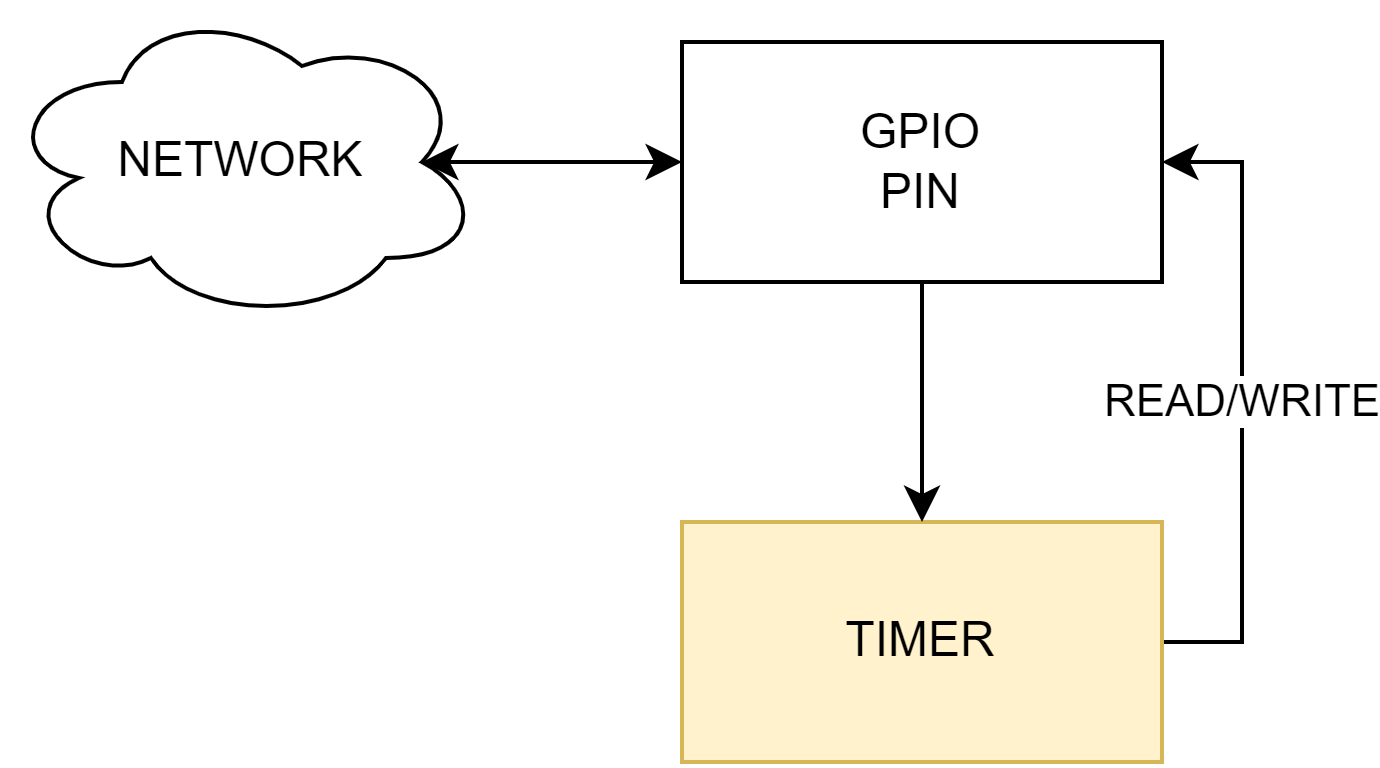
\psfig{file=Images/PhysicalReadIdealApproach.png,width=0.45\textwidth}}
    \caption{\footnotesize \centering Physical Layer implementation idea}
    \label{fig:PhysicalReadIdealApproach}
  \end{figure}

\section{Layer diagram}
\label{sec:Layer diagram Phy}
As can be understood, the architecture of the physical layer is not particularly complex: it receives data from the communication layer and broadcasts it to the network, and receives broadcast data from the network and forwards it to the communication layer. It can thus be schematized as follows:
  \begin{figure}[H]
    \centerline{
\psfig{file=Images/PhysicalLayerDiagram.png,width=0.5\textwidth}}
    \caption{\footnotesize \centering Physical Layer diagram}
    \label{fig:PhysicalLayerDiagram}
  \end{figure}

\section{Real implementation of the layer}
\label{sec:Real implementation of the layer Phy}
In the first section of this chapter, a possible implementation of the layer was provided. However, the proposed implementation is particularly complex to implement in practice.
Therefore, the choice was to use one of the UART modules on the MSP430 board to manage the sending and receiving of packets. 
The UART (Universal Asynchronous Receiver-Transmitter) module enables asynchronous communication that is not dependent on a synchronized clock and operates in full-duplex mode if necessary. It needs a dedicated TX output and RX input, which can be identified on the datasheet of the board.
Before the start of sending and receiving data, is needed to set the UART module to the desired baud rate. The baud rate indicates the transmission rate. Since is not present a shared clock it is necessary to have the same baud rate on the transmitting node and the receiving node to know how often to send and sample the signal.
For this project, the UART module was set to have a baud rate of 115200 b/s and send one byte at a time of data plus two bits to notify the start and end of the transmission.
The code below was used to achieve this configuration by taking the SMCLK (Sub-system master clock) set to 1MHz as the clock for baudrate generation.
\begin{lstlisting}
    //UART settings for BaudRate 115200 with 1MHz clock speed
    P2SEL0 &= ~(BIT5 | BIT6);
    P2SEL1 |= (BIT5 | BIT6);

    UCA1CTLW0 = UCSWRST;            //Put module in reset
    UCA1CTLW0 |= UCSSEL__SMCLK;
    UCA1BRW = 8;
    UCA1MCTLW = 0xD600;
    UCA1CTLW0 &= ~UCSWRST;          //Restore module from reset

    UCA1IE |= UCRXIE;               //Activate interrupt on module
\end{lstlisting}
RX TODO\\
TX TODO\\
  
\newpage





      \chapter{Evaluation}
The system presented exploits non-volatile memory to save data to be retained in the event of a power failure. The novelty of this implementation is the resistance to data loss in case of power failure added to the implementation of the TRAP protocol to reduce this type of events. To better highlight this progress, this chapter mainly presents some emulations performed with the presented stack, compared with emulations without the provided implementation.
\label{cha:Evaluation}
%memory overhead of implementation
\section{Technical details}
\label{sec:Technical deatils}
The size of the implementation varies according to the number of nodes within the network, the size of the RX and TX buffers saved in FRAM, and the optimization required of the compiler. 
For compiling optimization the highest level (Whole Program Optimization) is used, this also helps to reduce the power consumption of the system \cite{OptimizationCompiler}.\\
To provide some data, with 2 nodes in the network and the receive and send buffer (buffer RX and buffer TX) of size 3, the memory overhead is 5223 bytes.\\
The figure below shows the memory allocation provided by the Code Composer Studio IDE.\\
\begin{figure}[H]
\centerline{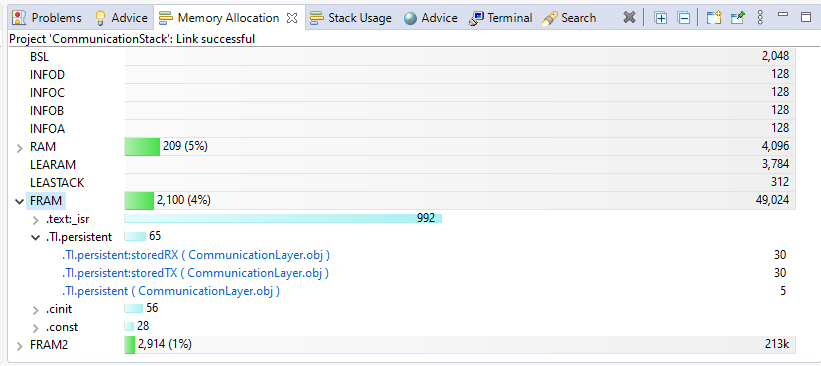
\psfig{file=Images/memoryOverhead.png,width=0.7\textwidth}}
\caption{\footnotesize \centering Memory overhead for network with 2 nodes and buffer size 3}
\label{fig:memoryOverhead}
\end{figure}
If the network nodes are increased to 16 and the size of both buffers to 32, the overhead will be 5307 bytes.\\
It is then possible to estimate the memory overhead of the implementation at about 5.5KB.
\section{Emulation}
\label{sec:Simulation}
The setup used for the emulations involves communication between two nodes; consequently, two TI MSP430 boards were used:
\begin{enumerate}
\item TI MSP430FR5994
\item TI MSP430FR5969
\end{enumerate}
For communication regarding the energy level (TRAP Layer), the backscatter channel was emulated using a wired connection. However, the operation is similar to using RF for transmission; in fact, it is based on toggling a GPIO pin for sending and generating external GPIO interrupts for receiving.\\
Communication between nodes for sending data is via the UART and is therefore also wired.\\
The choice to use UART rather than a GPIO pin to send the packet bit by bit was dictated by the difficulty of managing the latter implementation. Using a GPIO pin and sending either a high value or a low value depending on the bit value of the sequence to be sent would require sampling the signal at the sending frequency. This would result in adding complexity to the system.\\
In any case, since the communication stack presented is modular, replacement of the Physical Layer from UART to an implementation working with other types of communications does not require modification of the upper layers.\\
To observe the behavior of the nodes, a wired connection was made between the computer and the boards through another UART.\\\\
Tests consist of 20 minutes of emulated system operation;
it is important to note that these tests are limited to a short period of time and to limited cases. In order to get a more realistic overview of system performance, longer tests need to be conducted.\\
\begin{figure}[H]
\centerline{\psfig{file=Images/testBed.jpg,width=0.7\textwidth}}
\caption{\footnotesize \centering Test bed with MSP430FR5994 on the left and MSP430FR5969 on the right, white wires are for TRAP Layer, red wires are for data transmission}
\label{fig:testBed}
\end{figure}
\subsection{Energy Params For Emulation}
During the emulations, we do not have a system that can collect energy from its surroundings; therefore, the node capacitor is charged by a power source based on a random generation function.\\
The average percent increase in capacitor charge per second is declared before the test results.\\
Capacitor energy is consumed for data collection from the environment and forwarding to the application layer; this consumption during the emulation is fixed at 32\% of the maximum capacity.\\
Data transmission requires, in this emulation, a charge level of 64\% or more of the maximum capacitance of the capacitor, unlike reception, for which consumption of 62\% of the capacitance of the capacitor is simulated.\\
These estimated consumption values were decided by taking as reference a 2mF capacitor, a BGM220S BLE module \cite{BLEModule} for transmission, and a DHT11 humidity and temperature sensor \cite{DHT11Module} to collect the data from the surrounding environment.\\
Compared to SRAM, FRAM access results in a somewhat higher power consumption \cite{MSP430FRAMDS}, so when the stack is used, an additional 1\% consumption will be added to these values. In fact, the FRAM is used in receiving to save the data, in sending to retrieve the data, and in producing the packet to do the saving.\\
It is important to point out that the values presented are used only for emulation and do not reflect exactly the real capacitor capacity and consumption of the board.\\
When the simulated charge level of the capacitor reaches 0\%, the node is reset. To reset the node, an instruction from an invalid memory allocation is fetched.\\
Energy status update period is set to 1. This data item indicates every when the node energy information is sent to the network.
\subsection{Production Of Packages During The Emulation}
Data production on the nodes was simulated at fixed intervals, the emulations were performed with two different production patterns.\\
For the first test group, data was produced repeatedly every 60 seconds on the first node and every 90 seconds on the second node.\\
For the second test group, data was produced repeatedly every 60 seconds on the first node and every 75 seconds on the second.\\
This is useful for understanding the performance of the system with different production patterns.
\subsection{First test group}
\label{sec:FT}
In this first set of emulations, the operation of the system with and without the presented stack is tested. The energy level of the nodes is sent via Layer TRAP, and packets are produced repeatedly every 60 seconds on one node and every 90 seconds on the other.\\
Summary of the parameters of the emulation group:\\\\
\begin{tabular}{lll} \hline
Packet production repetition time on node 1: & 60 seconds\\ \hline
Packet production repetition time on node 2: & 90 seconds\\ \hline
Energy status update period: & 1 second \\ \hline
Simulated energy consumption in TX: & 64\% (+1\% if the stack is used) \\ \hline
Simulated energy consumption in RX: & 62\% (+1\% if the stack is used)\\ \hline
Simulated energy consumption for packet production: & 32\% (+1\% if the stack is used)\\ \hline
\end{tabular}
\begin{enumerate}
\item First emulation: average energy increment 0.71\% per second\\
For the first test an average energy growth per second inside the capacitor of about 0.71\% is emulated.\\
The result with the stack presented shows the sending of 5 packets and the successful reception of 5 packets, as opposed to not using it with which a result of 8 packets sent and 0 packets received is obtained (Figure \ref{fig:FGFT0}).\\
The success rate is then 100\% using the stack and 0\% without using the presented implementation.\\
It is important to note that fewer packets are sent with the use of the stack than with emulation without the stack. This result is closely related to the delay introduced by the TRAP protocol to allow the nodes to reach the correct energy level before starting transmission.\\
However, it is certainly better to successfully transmit fewer packets than to send more packets but not be sure of correct reception by the receiving node.
\begin{figure}[H]
\centerline{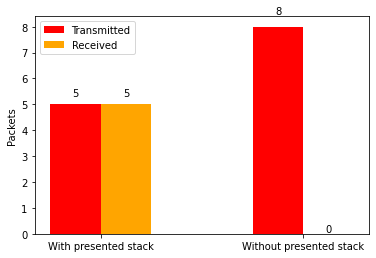
\psfig{file=Images/9060071MatPlot.png,width=0.5\textwidth}}\caption{\footnotesize \centering Emulation results with average energy increment of 0.71\% per second}
\label{fig:FGFT0}
\end{figure}
\begin{comment}
\begin{figure}[H]
\centerline{\psfig{file=Images/9060071RATIO.png,width=0.7\textwidth}}
\caption{\footnotesize \centering Success ratio of transmission with average energy increment of 0.71\% per second}
\label{fig:FGFT1}
\end{figure}
\end{comment}
\item Second emulation: average energy increment 1.25\% per second\\
This second emulation assumes an average energy growth of 1.25\% of the capacitor capacity per second.\\
If we go to analyze the data obtained from the tests, we can see that the results without using the stack are slightly better than what was seen in the previous emulations. This improvement is due to higher average energy growth.\\
In any case, the results obtained with the stack presented are still better than those obtained without using any protocol.
\begin{figure}[H]
\centerline{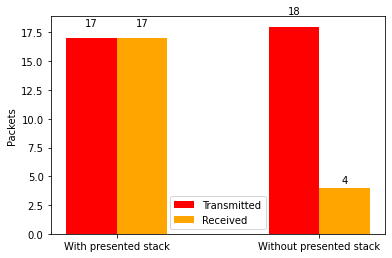
\psfig{file=Images/9060125MatPlot.png,width=0.5\textwidth}}
\caption{\footnotesize \centering Emulation results with average energy increment of 1.25\% per second}
\label{fig:FGST0}
\end{figure}
\begin{comment}
\begin{figure}[H]
\centerline{\psfig{file=Images/9060125RATIO.png,width=0.7\textwidth}}
\caption{\footnotesize \centering Success ratio of transmission with average energy increment of 1.25\% per second}
\label{fig:FGST1}
\end{figure}
\end{comment}
\item Third emulation: average energy increment 2\% per second\\
Following the trend of previous tests, the average value of per-second increment of energy within the capacitor is also changed in these emulations. In particular, an average increment of 2\% is proposed.\\
Similar to what highlighted in the previous test, the result without the stack achieves a higher transmission success rate than the first case presented, this increase is due to a higher growth of the energy inside the capacitor.\\
However, the stack allows the system to achieve better performance.\\
It is interesting to note that, during this emulation, the number of total transmissions using the stack is higher than the number of transmissions without the stack (Figure \ref{fig:FGTT0}). This increase in transmissions is due to the saving of packets already produced in non-volatile memory and consequently as soon as possible the saved packets are sent without waiting for a new production.
\begin{figure}[H]
\centerline{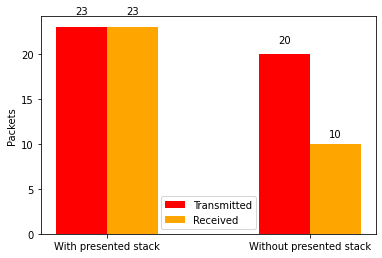
\psfig{file=Images/90602MatPlot.png,width=0.5\textwidth}}
\caption{\footnotesize \centering Emulation results with average energy increment of 2\% per second}
\label{fig:FGTT0}
\end{figure}
\begin{comment}
\begin{figure}[H]
\centerline{\psfig{file=Images/90602RATIO.png,width=0.7\textwidth}}
\caption{\footnotesize \centering Success ratio of transmission with average energy increment of 2\% per second}
\label{fig:FGTT1}
\end{figure}
\end{comment}
\end{enumerate}
\newpage
\subsection{Second test group}
\label{sec:ST}
This second group of emulations follows the same energy pattern presented with the previous group; however, having different periods for packet production the results obtained in relation to the number of transmissions are slightly different. The production periods are set to 60 seconds for the first node and 75 seconds for the second.\\
Summary of the parameters of the emulation group:\\\\
\begin{tabular}{lll} \hline
Packet production repetition time on node 1: & 60 seconds\\ \hline
Packet production repetition time on node 2: & 75 seconds\\ \hline
Energy status update period: & 1 second \\ \hline
Simulated energy consumption in TX: & 64\% (+1\% if the stack is used)\\ \hline
Simulated energy consumption in RX: & 62\% (+1\% if the stack is used)\\ \hline
Simulated energy consumption for packet production: & 32\% (+1\% if the stack is used)\\ \hline
\end{tabular}
\begin{enumerate}
\item First emulation: average energy increment 0.71\% per second\\
The first emulation assumes a percentage energy growth of 0.71\% of the capacitor capacity per second.\\
It can be seen from the results obtained that the number of successful transmissions is significantly higher if the presented stack is used (Figure \ref{fig:SGFT0}).\\
The result is particularly significant in that it shows that, in the case of low energy growth within the node, the presented stack, due to the implementation of the TRAP protocol, performs better than not using any control during transmission.\\
Again, the lower number of transmission actions observable with the use of the stack is due to the TRAP protocol delaying sending until the energy levels required to successfully complete the transmission are reached.
\begin{figure}[H]
\centerline{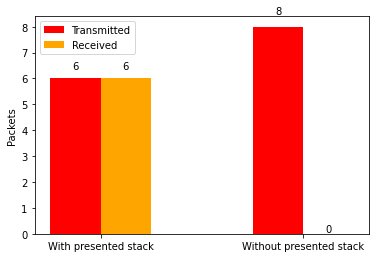
\psfig{file=Images/7560071MatPlot.png,width=0.5\textwidth}}
\caption{\footnotesize \centering Emulation results with average energy increment of 0.71\% per second}
\label{fig:SGFT0}
\end{figure}
\begin{comment}
\begin{figure}[H]
\centerline{\psfig{file=Images/7560071RATIO.png,width=0.7\textwidth}}
\caption{\footnotesize \centering Success ratio of transmission with average energy increment of 0.71\% per second}
\label{fig:SGFT1}
\end{figure}
\end{comment}
\item Second emulation: average energy increment 1.25\% per second\\
Also in this tests, results obtained with the stack are better in relation to the one without.\\
However, it is interesting to note that, with a higher energy growth than in the previous test, more packets can be sent using the stack. This increase is due to the use of FRAM memory by the stack, which then creates a persistent queue of packets to be sent that is not dropped on power failure.
\begin{figure}[H]
\centerline{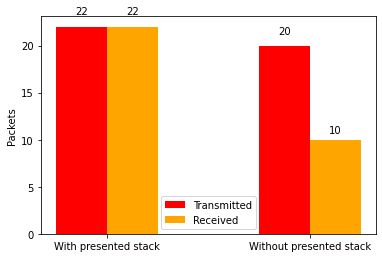
\psfig{file=Images/7560125MatPlot.png,width=0.5\textwidth}}
\caption{\footnotesize \centering Emulation results with average energy increment of 1.25\% per second}
\label{fig:SGST0}
\end{figure}
\begin{comment}
\begin{figure}[H]
\centerline{\psfig{file=Images/7560125RATIO.png,width=0.7\textwidth}}
\caption{\footnotesize \centering Success ratio of transmission with average energy increment of 1.25\% per second}
\label{fig:SGST1}
\end{figure}
\end{comment}
\item Third emulation: average energy increment 2\% per second\\
The third test presents very similar results (Figure \ref{fig:SGTT0}) to those described in the second test (Figure \ref{fig:SGST0}), also in this emulation the success ratio of the stack is 100\% as opposed to the one without the stack which is significantly lower (about 37\%).\\
We can also highlight in this test the higher number of packets sent using the stack despite the delay in transmission introduced by the TRAP protocol to achieve the energy levels required for successful transmission.
\begin{figure}[H]
\centerline{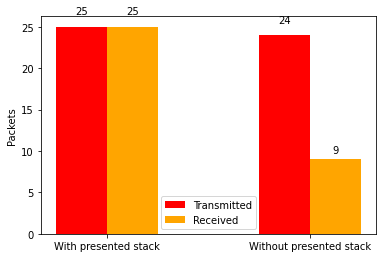
\psfig{file=Images/75602MatPlot.png,width=0.5\textwidth}}
\caption{\footnotesize \centering Emulation results with average energy increment of 2\% per second}
\label{fig:SGTT0}
\end{figure}
\begin{comment}
\begin{figure}[H]
\centerline{\psfig{file=Images/7560125RATIO.png,width=0.7\textwidth}}
\caption{\footnotesize \centering Success ratio of transmission with average energy increment of 2\% per second}
\label{fig:SGTT1}
\end{figure}
\end{comment}
\end{enumerate}
\section{Results Discussion}
\label{sec:SimulationDiscussion}
The tests carried out showed that in the case of using the stack presented in this thesis, the performance of the system in terms of successfully sent packets goes up significantly.\\
Calculating an average relative to the success rate obtained with the stack we observe that is almost 70 percentage points higher than the result obtained without the use of any protocol (Figures \ref{fig:FTA}).

\begin{figure}[H]
\centerline{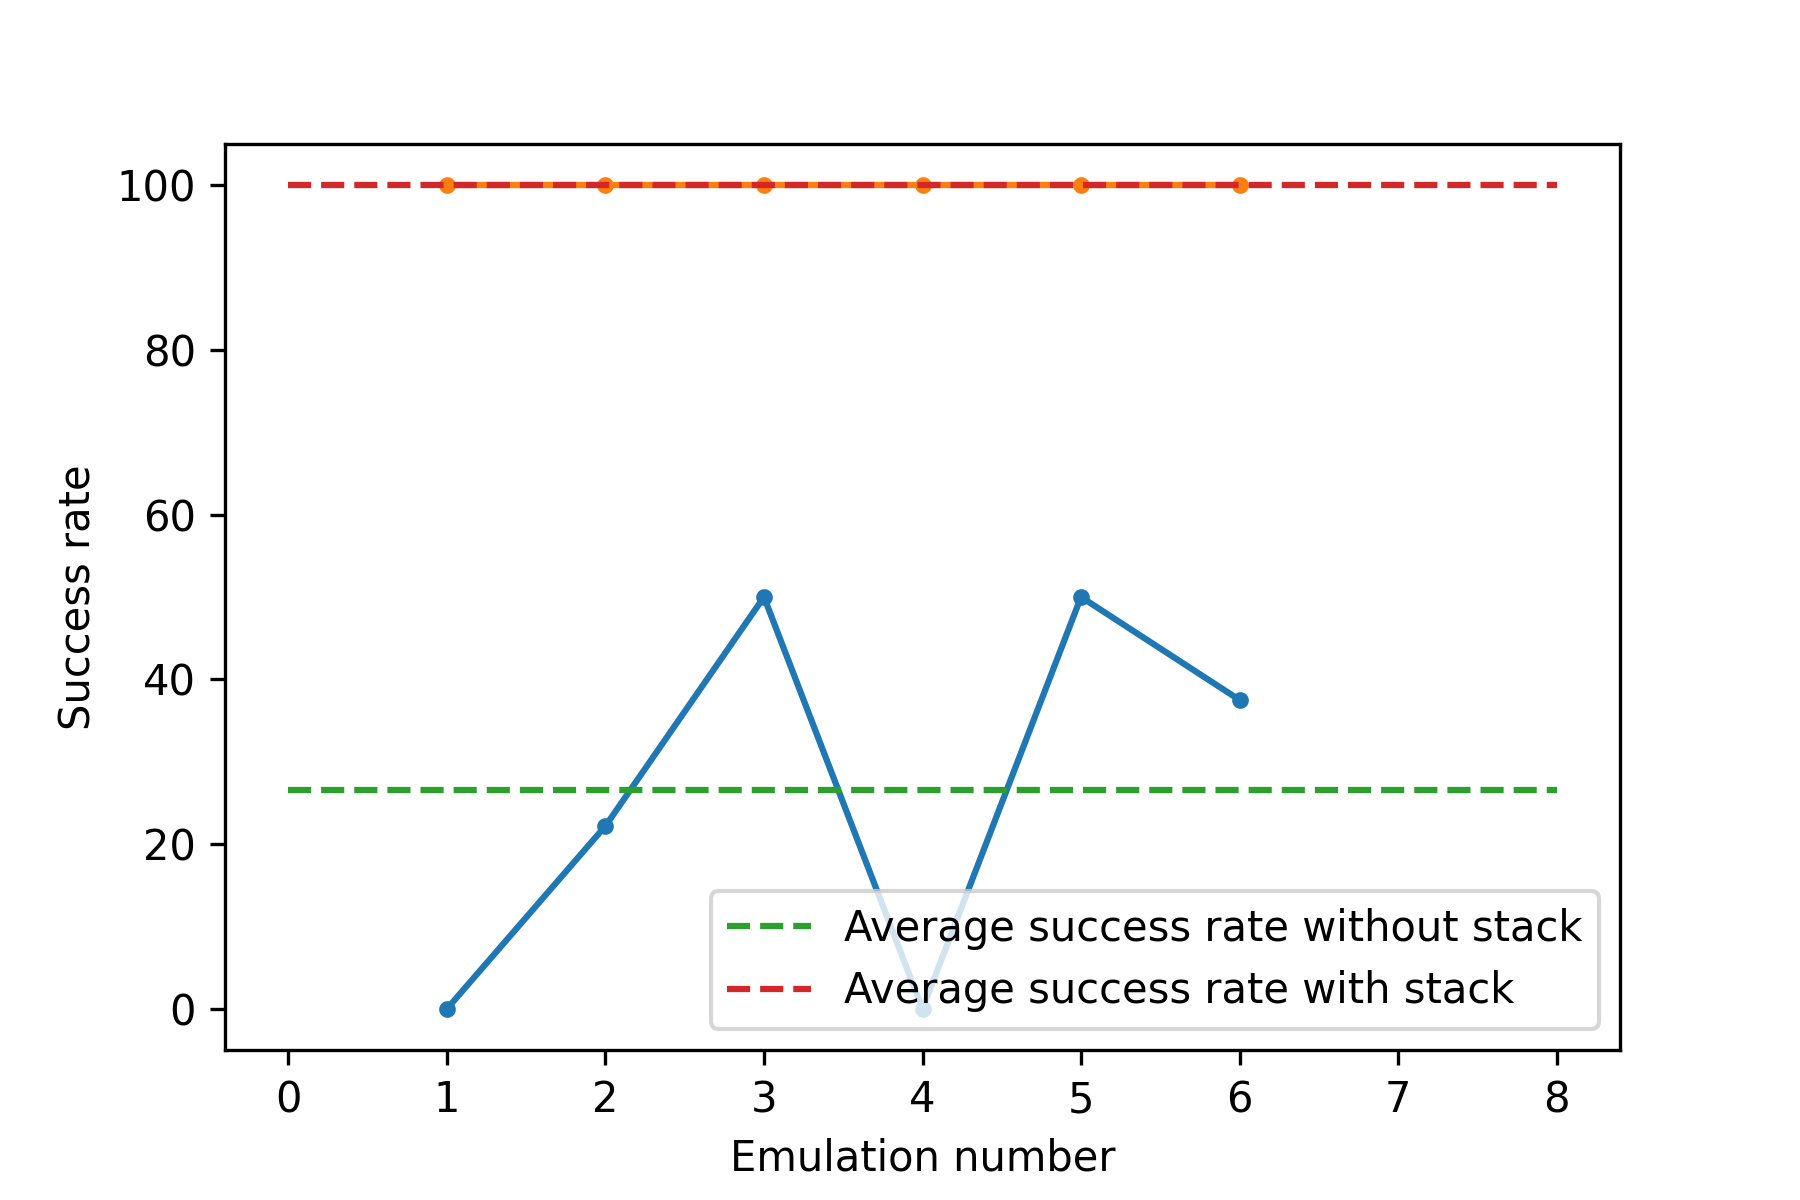
\psfig{file=Images/finalAverage.png,width=0.7\textwidth}}
\caption{\footnotesize \centering Plot representing the success rate in transmission obtained with and without the presented stack. The dashed line represents the average value obtained. The stack improves system performance by almost 70\%.}
\label{fig:FTA}
\end{figure}

In particular, it can be seen that under conditions in which the capacitor is charged by an energy source capable of providing only a small percentage charge per second (Figure \ref{fig:FGFT0} and Figure \ref{fig:SGFT0}) the performance of the system using the presented stack is very good in relation to the number of packets successfully sent.\\
This improvement is mainly due to the use of the TRAP protocol to make the node aware of the energy level of neighboring nodes and thus avoid wasting energy on transmissions that cannot be completed.\\\\
It is important to remember how the tests were not run for long periods of time and how they did not take into account all possible situations that the system might encounter during ordinary operation. However, they do allow for a general idea regarding the performance of the system with and without the use of the presented stack.
\newpage





      \chapter{Conclusion And Future Work}
\label{cha:conclusion}
\section{Conclusion}
In this thesis, a tiny network stack for battery-free communication is designed, implemented and evaluated.\\
The presented system is published in an open source manner at the project's GitHub page \footnote{https://github.com/cancianilorenzo/Tiny-network-stack-for-battery-free-communication} where it is also possible to find up-to-date documentation.\\
The stack has the features required in Chapter 1, thus saving data in non-volatile memory, retrieving it to perform sending to the network nodes or to the Application Layer to process it, recognizing expired packets to avoid wasting energy in sending/receiving invalid data, and implementing the TRAP protocol to make nodes aware about the energy available on neighboring nodes.\\
In addition to this, the presented system is modular in that it adapts to different transmission technologies by replacing only the Physical Layer and is scalable since it is not tied to a fixed number of nodes in the network.\\
Another feature of the system presented is that it hides implementation complexity from the Application Layer. For this reason, the system exposes only a small set of functions that can be used by the Application Layer. An example of its use is as follows:\\
\begin{lstlisting}
....
while (1)
{
    dataProduced(datax, datay, dataj, dataz, destinationNode);
    dataSend();
    storedData dataRec = getData();

}
....
\end{lstlisting}
From the evaluation chapter, it was found that the results obtained with the presented stack are better than not using any protocol. In fact, the transmission success rate stands at 100\% if the stack is used, around 26\% if it is not used.\\
In addition to the loss of data in transmission the stack helps to reduce energy waste, in fact it is important to note that all packets sent and not received due to low energy on the receiving node meant a loss for both nodes: the sending node lost energy for producing and sending the data, while the receiving node lost energy for receiving a portion of the packet.

\section{Future Work}
Due to lack of time (tests on real data are usually very demanding and take several days to complete a single trial), numerous modifications, tests and experiments have been postponed. Future research will focus on deepening certain mechanisms, new suggestions for testing, new implementation techniques, or simple curiosity to develop something ever better.

\newpage
      %\input{capitolo4}
      
      
    \endgroup


    % bibliografia in formato bibtex
    %
    % aggiunta del capitolo nell'indice
    \addcontentsline{toc}{chapter}{Bibliography}
    % stile con ordinamento alfabetico in funzione degli autori
    \bibliographystyle{plain}
    \bibliography{biblio}
%%%%%%%%%%%%%%%%%%%%%%%%%%%%%%%%%%%%%%%%%%%%%%%%%%%%%%%%%%%%%%%%%%%%%%%%%%
%%%%%%%%%%%%%%%%%%%%%%%%%%%%%%%%%%%%%%%%%%%%%%%%%%%%%%%%%%%%%%%%%%%%%%%%%%
%% Nota
%%%%%%%%%%%%%%%%%%%%%%%%%%%%%%%%%%%%%%%%%%%%%%%%%%%%%%%%%%%%%%%%%%%%%%%%%%
%% Nella bibliografia devono essere riportati tutte le fonti consultate 
%% per lo svolgimento della tesi. La bibliografia deve essere redatta 
%% in ordine alfabetico sul cognome del primo autore. 
%% 
%% La forma della citazione bibliografica va inserita secondo la fonte utilizzata:
%% 
%% LIBRI
%% Cognome e iniziale del nome autore/autori, la data di edizione, titolo, casa editrice, eventuale numero dell’edizione. 
%% 
%% ARTICOLI DI RIVISTA
%% Cognome e iniziale del nome autore/autori, titolo articolo, titolo rivista, volume, numero, numero di pagine.
%% 
%% ARTICOLI DI CONFERENZA
%% Cognome e iniziale del nome autore/autori (anno), titolo articolo, titolo conferenza, luogo della conferenza (città e paese), date della conferenza, numero di pagine. 
%% 
%% SITOGRAFIA
%% La sitografia contiene un elenco di indirizzi Web consultati e disposti in ordine alfabetico. 
%% E’ necessario:
%%   Copiare la URL (l’indirizzo web) specifica della pagina consultata
%%   Se disponibile, indicare il cognome e nome dell’autore, il titolo ed eventuale sottotitolo del testo
%%   Se disponibile, inserire la data di ultima consultazione della risorsa (gg/mm/aaaa).    
%%%%%%%%%%%%%%%%%%%%%%%%%%%%%%%%%%%%%%%%%%%%%%%%%%%%%%%%%%%%%%%%%%%%%%%%%%
%%%%%%%%%%%%%%%%%%%%%%%%%%%%%%%%%%%%%%%%%%%%%%%%%%%%%%%%%%%%%%%%%%%%%%%%%%
    

    \titleformat{\chapter}
        {\normalfont\Huge\bfseries}{Allegato \thechapter}{1em}{}
    % sezione Allegati - opzionale
    \appendix

\end{document}
